\documentclass[12pt, a4paper]{article}

\usepackage[dvips]{graphics}
\usepackage{tabularx}
\usepackage{amsmath}
\usepackage{amsfonts}
\usepackage{amssymb}
\usepackage{graphicx}
\usepackage{float}
\usepackage{listings}
\usepackage{rotating}
\usepackage{tikz}
\usepackage{verbatim}
\usepackage{csvsimple}
\usepackage{rotating}
\usepackage{changepage}
\pdfgentounicode=1

\lstset{
        basicstyle=\ttfamily\scriptsize,
        keywordstyle=\bfseries,
        showspaces=false,
        showstringspaces=false,
        morekeywords={*,IF,FOR, STRUCT, FUNCTION, INT, FLOAT, ELSE, RETURN, STOP, Frame, FMB, PROJ, ELIM_VAR},
        mathescape=true
    }

\begin{document}

\title{The FMB Algorithm}
\author{Pascal Baillehache\\bayashipascal@gmail.com}
\date{\today}
\maketitle
\begin{center}
\begin{figure}[H]
\centering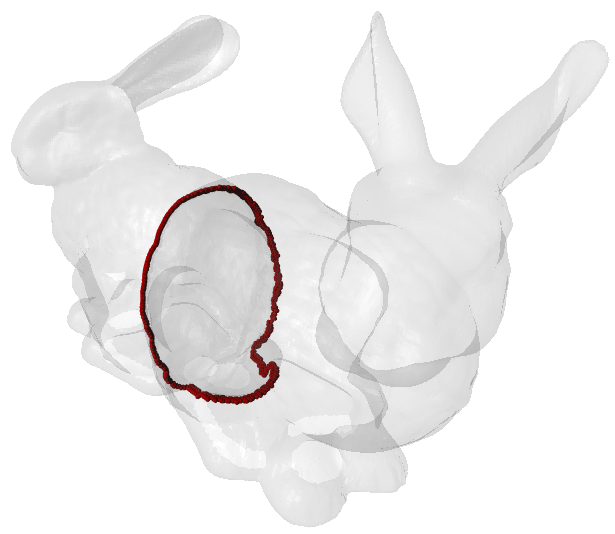
\includegraphics[width=5cm]{./bunny.png}\\
\end{figure}
\end{center}
\thispagestyle{empty}

\begin{abstract}
This paper introduces how to perform intersection detection of pair of static/dynamic cuboid/tetrahedron in 2D/3D by using the Fourier-Motzkin elimination method.\\
It includes the mathematical definition of the problem, its mathematical resolution with the Fourier-Motzkin elimination method, the resulting algorithm and its implementation in C, and its validation and qualification against the SAT algorithm. Results are commented and show that the FMB algorithm can be in average up to 4 times faster than the SAT algorithm.
\end{abstract}

\newpage
\tableofcontents

\section*{Introduction}

This paper introduces the FMB (Fourier-Motzkin-Baillehache) algorithm which can be used to perform intersection detection of moving and resting parallelepipeds and triangles in 2D, parallelepipeds and triangles in 3D, and cuboids and tetrahedrons in 3D.\\

The detection result is returned has a boolean (intersection / no intersection), and if there is intersection, a bounding box of the intersection.\\

The two first sections introduce how the problem can be expressed as a system of linear inequation, and its resolution using the Fourier-Motzkin method.\\

The algorithm of the solution and its implementation in the C programming language are detailed in the three following sections.\\

The three next sections introduce the unit tests, the validation and the qualification in term of relative performance of the FMB algorithm against the SAT algorithm.\\

Finally, the last section contains comments about the qualification results.\\

All the algorithms, the code, the results and this doc are available on GitHub at:
\begin{center}
https://github.com/BayashiPascal/FMB
 \end{center}
Please, make sure you have the most recent version of this paper by referring to the master branch of this repository.
 
\section{The problem as a system of linear inequations}

\subsection{Notations and definitions}

\begin{itemize}
\item{$\left[M\right]_{r,c}$ is the component at column $c$ and row $r$ of the matrix $M$}
\item{$\left[V\right]_r$ is the $r$-th component of the vector $\overrightarrow{V}$}
\item the term "Frame" is used indifferently for parallelepiped, triangle, cuboid and tetrahedron.
\end{itemize}

\subsection{Static case}

The two Frames are represented as a vector origin and a number of component vectors equal to the dimension $D$ of the space where live the Frames. Each vector is of dimension equal to $D$.\\

Let's call $\mathbb{A}$ and $\mathbb{B}$ the two Frames tested for intersection. If $\mathbb{A}$ and $\mathbb{B}$ are two cuboids:
\begin{equation}
\mathbb{A}=\left\lbrace
\begin{array}{c}
\overrightarrow{X}\in[0.0,1.0]^D\\
\overrightarrow{O_\mathbb{A}}+C_\mathbb{A}.\overrightarrow{X}
\end{array}
\right\rbrace
\end{equation}
\begin{equation}
\mathbb{B}=\left\lbrace
\begin{array}{c}
\overrightarrow{X}\in[0.0,1.0]^D\\
\overrightarrow{O_\mathbb{B}}+C_\mathbb{B}.\overrightarrow{X}
\end{array}
\right\rbrace
\end{equation}
where $\overrightarrow{O_\mathbb{A}}$ is the origin of $\mathbb{A}$ and $C_\mathbb{A}$ is the matrix of the components of $\mathbb{A}$ (one component per column). Idem for $\overrightarrow{O_\mathbb{B}}$ and $C_\mathbb{B}$.\\

If $\mathbb{A}$ and $\mathbb{B}$ are two tetrahedrons:
\begin{equation}
\mathbb{A}=\left\lbrace
\begin{array}{c}
\overrightarrow{X}\in[0.0,1.0]^D\\
\sum_{i=0}^{D-1}\left[X\right]_i\le1.0\\
\overrightarrow{O_\mathbb{A}}+C_\mathbb{A}.\overrightarrow{X}
\end{array}
\right\rbrace
\end{equation}
\begin{equation}
\mathbb{B}=\left\lbrace
\begin{array}{c}
\overrightarrow{X}\in[0.0,1.0]^D\\
\sum_{i=0}^{D-1}\left[X\right]_i\le1.0\\
\overrightarrow{O_\mathbb{B}}+C_\mathbb{B}.\overrightarrow{X}
\end{array}
\right\rbrace
\end{equation}

I'll assume the Frames are well formed, i.e. their components matrix is invertible. It is then possible to express $\mathbb{B}$ in $\mathbb{A}$'s coordinates system, noted as $\mathbb{B}_\mathbb{A}$. If $\mathbb{B}$ is a cuboid:
\begin{equation}
\mathbb{B}_\mathbb{A}=\left\lbrace
\begin{array}{c}
\overrightarrow{X}\in[0.0,1.0]^D\\
C_\mathbb{A}^{-1}.(\overrightarrow{O_\mathbb{B}}-\overrightarrow{O_\mathbb{A}}+C_\mathbb{B}.\overrightarrow{X})
\end{array}
\right\rbrace
\end{equation}

If $\mathbb{B}$ is a tetrahedron:
\begin{equation}
\mathbb{B}_\mathbb{A}=\left\lbrace
\begin{array}{c}
\overrightarrow{X}\in[0.0,1.0]^D\\
\sum_{i=0}^{D-1}\left[X\right]_i\le1.0\\
C_\mathbb{A}^{-1}.(\overrightarrow{O_\mathbb{B}}-\overrightarrow{O_\mathbb{A}}+C_\mathbb{B}.\overrightarrow{X})
\end{array}
\right\rbrace
\end{equation}

$\mathbb{A}$ in its own coordinates system becomes, for a cuboid:
\begin{equation}
\mathbb{A}_\mathbb{A}=\left\lbrace\overrightarrow{X}\in[0.0,1.0]^D\right\rbrace
\end{equation}

and for a tetrahedron:
\begin{equation}
\mathbb{A}_\mathbb{A}=\left\lbrace
\begin{array}{c}
\overrightarrow{X}\in[0.0,1.0]^D\\
\sum_{i=0}^{D-1}\left[X\right]_i\le1.0
\end{array}
\right\rbrace
\end{equation}

The intersection of $\mathbb{A}$ and $\mathbb{B}$ in $\mathbb{A}$'s coordinates sytem, $\mathbb{A}_\mathbb{A}\cap\mathbb{B}_\mathbb{A}$,can then be expressed as follow.\\

If $\mathbb{A}$ and $\mathbb{B}$ are two cuboids:
\begin{equation}
\mathbb{A}_\mathbb{A}\cap\mathbb{B}_\mathbb{A}=\left\lbrace
\begin{array}{c}
\overrightarrow{X}\in[0.0,1.0]^D\\
C_\mathbb{A}^{-1}.\left(\overrightarrow{O_\mathbb{B}}-\overrightarrow{O_\mathbb{A}}+C_\mathbb{B}.\overrightarrow{X}\right)\cap[0.0,1.0]^D
\end{array}
\right\rbrace
\end{equation}

If $\mathbb{A}$ is a cuboid and $\mathbb{B}$ is a tetrahedron:
\begin{equation}
\mathbb{A}_\mathbb{A}\cap\mathbb{B}_\mathbb{A}=\left\lbrace
\begin{array}{c}
\overrightarrow{X}\in[0.0,1.0]^D\\
\sum_{i=0}^{D-1}\left[X\right]_i\le1.0\\
C_\mathbb{A}^{-1}.\left(\overrightarrow{O_\mathbb{B}}-\overrightarrow{O_\mathbb{A}}+C_\mathbb{B}.\overrightarrow{X}\right)\cap[0.0,1.0]^D
\end{array}
\right\rbrace
\end{equation}

If $\mathbb{A}$ is a tetrahedron and $\mathbb{B}$ is a cuboid:
\begin{equation}
\mathbb{A}_\mathbb{A}\cap\mathbb{B}_\mathbb{A}=\left\lbrace
\begin{array}{c}
\overrightarrow{X}\in[0.0,1.0]^D\\
C_\mathbb{A}^{-1}.\left(\overrightarrow{O_\mathbb{B}}-\overrightarrow{O_\mathbb{A}}+C_\mathbb{B}.\overrightarrow{X}\right)\cap[0.0,1.0]^D\\
\sum_{i=0}^{D-1}\left[C_\mathbb{A}^{-1}.\left(\overrightarrow{O_\mathbb{B}}-\overrightarrow{O_\mathbb{A}}+C_\mathbb{B}.\overrightarrow{X}\right)\right]_i\le1.0\\
\end{array}
\right\rbrace
\end{equation}

If $\mathbb{A}$ and $\mathbb{B}$ are two tetrahedrons:
\begin{equation}
\mathbb{A}_\mathbb{A}\cap\mathbb{B}_\mathbb{A}=\left\lbrace
\begin{array}{c}
\overrightarrow{X}\in[0.0,1.0]^D\\
\sum_{i=0}^{D-1}\left[X\right]_i\le1.0\\
C_\mathbb{A}^{-1}.(\overrightarrow{O_\mathbb{B}}-\overrightarrow{O_\mathbb{A}}+C_\mathbb{B}.\overrightarrow{X})\cap[0.0,1.0]^D\\
\sum_{i=0}^{D-1}\left[C_\mathbb{A}^{-1}.\left(\overrightarrow{O_\mathbb{B}}-\overrightarrow{O_\mathbb{A}}+C_\mathbb{B}.\overrightarrow{X}\right)\right]_i\le1.0\\
\end{array}
\right\rbrace
\end{equation}

These can in turn be expressed as systems of linear inequations as follow, given the two shortcuts $\overrightarrow{O_{\mathbb{B}_\mathbb{A}}}=C_\mathbb{A}^{-1}.(\overrightarrow{O_\mathbb{B}}-\overrightarrow{O_\mathbb{A}})$ and $C_{\mathbb{B}_\mathbb{A}}=C_\mathbb{A}^{-1}.C_{\mathbb{B}}$.

If $\mathbb{A}$ and $\mathbb{B}$ are two cuboids:
\begin{equation}
\left\lbrace
\begin{array}{rcl}
\left[X\right]_0&\le&1.0\\
...\\
\left[X\right]_{D-1}&\le&1.0\\
-\left[X\right]_0&\le&0.0\\
...\\
-\left[X\right]_{D-1}&\le&0.0\\
\sum_{i=0}^{D-1}\left[C_{\mathbb{B}_\mathbb{A}}\right]_{i,0}.\left[X\right]_i&\le&1.0-\left[O_{\mathbb{B}_\mathbb{A}}\right]_0\\
...\\
\sum_{i=0}^{D-1}\left[C_{\mathbb{B}_\mathbb{A}}\right]_{i,D-1}.\left[X\right]_i&\le&1.0-\left[O_{\mathbb{B}_\mathbb{A}}\right]_{D-1}\\
-\sum_{i=0}^{D-1}\left[C_{\mathbb{B}_\mathbb{A}}\right]_{i,0}.\left[X\right]_i&\le&\left[O_{\mathbb{B}_\mathbb{A}}\right]_0\\
...\\
-\sum_{i=0}^{D-1}\left[C_{\mathbb{B}_\mathbb{A}}\right]_{i,D-1}.\left[X\right]_i&\le&\left[O_{\mathbb{B}_\mathbb{A}}\right]_{D-1}
\end{array}
\right.
\end{equation}

If $\mathbb{A}$ is a cuboid and $\mathbb{B}$ is a tetrahedron:
\begin{equation}
\left\lbrace
\begin{array}{rcl}
-\left[X\right]_0&\le&0.0\\
...\\
-\left[X\right]_{D-1}&\le&0.0\\
\sum_{i=0}^{D-1}\left[C_{\mathbb{B}_\mathbb{A}}\right]_{i,0}.\left[X\right]_i&\le&1.0-\left[O_{\mathbb{B}_\mathbb{A}}\right]_0\\
...\\
\sum_{i=0}^{D-1}\left[C_{\mathbb{B}_\mathbb{A}}\right]_{i,D-1}.\left[X\right]_i&\le&1.0-\left[O_{\mathbb{B}_\mathbb{A}}\right]_{D-1}\\
-\sum_{i=0}^{D-1}\left[C_{\mathbb{B}_\mathbb{A}}\right]_{i,0}.\left[X\right]_i&\le&\left[O_{\mathbb{B}_\mathbb{A}}\right]_0\\
...\\
-\sum_{i=0}^{D-1}\left[C_{\mathbb{B}_\mathbb{A}}\right]_{i,D-1}.\left[X\right]_i&\le&\left[O_{\mathbb{B}_\mathbb{A}}\right]_{D-1}\\
\sum_{i=0}^{D-1}\left[X\right]_i&\le&1.0
\end{array}
\right.
\end{equation}

If $\mathbb{A}$ is a tetrahedron and $\mathbb{B}$ is a cuboid:
\begin{equation}
\left\lbrace
\begin{array}{rcl}
\left[X\right]_0&\le&1.0\\
...\\
\left[X\right]_{D-1}&\le&1.0\\
-\left[X\right]_0&\le&0.0\\
...\\
-\left[X\right]_{D-1}&\le&0.0\\
-\sum_{i=0}^{D-1}\left[C_{\mathbb{B}_\mathbb{A}}\right]_{i,0}.\left[X\right]_i&\le&\left[O_{\mathbb{B}_\mathbb{A}}\right]_0\\
...\\
-\sum_{i=0}^{D-1}\left[C_{\mathbb{B}_\mathbb{A}}\right]_{i,D-1}.\left[X\right]_i&\le&\left[O_{\mathbb{B}_\mathbb{A}}\right]_{D-1}\\
\sum_{j=0}^{D-1}\left(\sum_{i=0}^{D-1}\left[C_{\mathbb{B}_\mathbb{A}}\right]_{i,j}.\left[X\right]_i\right)&\le&1.0-\sum_{j=0}^{D-1}\left[O_{\mathbb{B}_\mathbb{A}}\right]_j
\end{array}
\right.
\end{equation}

If $\mathbb{A}$ and $\mathbb{B}$ are two tetrahedrons:
\begin{equation}
\left\lbrace
\begin{array}{rcl}
-\left[X\right]_0&\le&0.0\\
...\\
-\left[X\right]_{D-1}&\le&0.0\\
-\sum_{i=0}^{D-1}\left[C_{\mathbb{B}_\mathbb{A}}\right]_{i,0}.\left[X\right]_i&\le&\left[O_{\mathbb{B}_\mathbb{A}}\right]_0\\
...\\
-\sum_{i=0}^{D-1}\left[C_{\mathbb{B}_\mathbb{A}}\right]_{i,D-1}.\left[X\right]_i&\le&\left[O_{\mathbb{B}_\mathbb{A}}\right]_{D-1}\\
\sum_{i=0}^{D-1}\left[X\right]_i&\le&1.0\\
\sum_{j=0}^{D-1}\left(\sum_{i=0}^{D-1}\left[C_{\mathbb{B}_\mathbb{A}}\right]_{i,j}.\left[X\right]_i\right)&\le&1.0-\sum_{j=0}^{D-1}\left[O_{\mathbb{B}_\mathbb{A}}\right]_j
\end{array}
\right.
\end{equation}

If one wants to consider faces (parallelepipeds and triangles) in 3D, by assuming the third component of cuboid and tetrahedron is the normal of the faces, she can simply modifies the inequations above to express the constraint $X_2=0$ and obtain the relevant systems as follow.

If $\mathbb{A}$ and $\mathbb{B}$ are two cuboids:
\begin{equation}
\left\lbrace
\begin{array}{rcl}
\left[X\right]_0&\le&1.0\\
...\\
\left[X\right]_{D-2}&\le&1.0\\
-\left[X\right]_0&\le&0.0\\
...\\
-\left[X\right]_{D-2}&\le&0.0\\
\sum_{i=0}^{D-2}\left[C_{\mathbb{B}_\mathbb{A}}\right]_{i,0}.\left[X\right]_i&\le&1.0-\left[O_{\mathbb{B}_\mathbb{A}}\right]_0\\
...\\
\sum_{i=0}^{D-2}\left[C_{\mathbb{B}_\mathbb{A}}\right]_{i,D-2}.\left[X\right]_i&\le&1.0-\left[O_{\mathbb{B}_\mathbb{A}}\right]_{D-2}\\
\sum_{i=0}^{D-2}\left[C_{\mathbb{B}_\mathbb{A}}\right]_{i,D-1}.\left[X\right]_i&\le&-\left[O_{\mathbb{B}_\mathbb{A}}\right]_{D-1}\\
-\sum_{i=0}^{D-2}\left[C_{\mathbb{B}_\mathbb{A}}\right]_{i,0}.\left[X\right]_i&\le&\left[O_{\mathbb{B}_\mathbb{A}}\right]_0\\
...\\
-\sum_{i=0}^{D-2}\left[C_{\mathbb{B}_\mathbb{A}}\right]_{i,D-1}.\left[X\right]_i&\le&\left[O_{\mathbb{B}_\mathbb{A}}\right]_{D-1}
\end{array}
\right.
\end{equation}

If $\mathbb{A}$ is a cuboid and $\mathbb{B}$ is a tetrahedron:
\begin{equation}
\left\lbrace
\begin{array}{rcl}
-\left[X\right]_0&\le&0.0\\
...\\
-\left[X\right]_{D-2}&\le&0.0\\
\sum_{i=0}^{D-2}\left[C_{\mathbb{B}_\mathbb{A}}\right]_{i,0}.\left[X\right]_i&\le&1.0-\left[O_{\mathbb{B}_\mathbb{A}}\right]_0\\
...\\
\sum_{i=0}^{D-2}\left[C_{\mathbb{B}_\mathbb{A}}\right]_{i,D-2}.\left[X\right]_i&\le&1.0-\left[O_{\mathbb{B}_\mathbb{A}}\right]_{D-2}\\
\sum_{i=0}^{D-2}\left[C_{\mathbb{B}_\mathbb{A}}\right]_{i,D-1}.\left[X\right]_i&\le&-\left[O_{\mathbb{B}_\mathbb{A}}\right]_{D-1}\\
-\sum_{i=0}^{D-2}\left[C_{\mathbb{B}_\mathbb{A}}\right]_{i,0}.\left[X\right]_i&\le&\left[O_{\mathbb{B}_\mathbb{A}}\right]_0\\
...\\
-\sum_{i=0}^{D-2}\left[C_{\mathbb{B}_\mathbb{A}}\right]_{i,D-1}.\left[X\right]_i&\le&\left[O_{\mathbb{B}_\mathbb{A}}\right]_{D-1}\\
\sum_{i=0}^{D-2}\left[X\right]_i&\le&1.0
\end{array}
\right.
\end{equation}

If $\mathbb{A}$ is a tetrahedron and $\mathbb{B}$ is a cuboid:
\begin{equation}
\left\lbrace
\begin{array}{rcl}
\left[X\right]_0&\le&1.0\\
...\\
\left[X\right]_{D-2}&\le&1.0\\
-\left[X\right]_0&\le&0.0\\
...\\
-\left[X\right]_{D-2}&\le&0.0\\
-\sum_{i=0}^{D-2}\left[C_{\mathbb{B}_\mathbb{A}}\right]_{i,0}.\left[X\right]_i&\le&\left[O_{\mathbb{B}_\mathbb{A}}\right]_0\\
...\\
-\sum_{i=0}^{D-2}\left[C_{\mathbb{B}_\mathbb{A}}\right]_{i,D-1}.\left[X\right]_i&\le&\left[O_{\mathbb{B}_\mathbb{A}}\right]_{D-1}\\
\sum_{j=0}^{D-2}\left(\sum_{i=0}^{D-2}\left[C_{\mathbb{B}_\mathbb{A}}\right]_{i,j}.\left[X\right]_i\right)&\le&1.0-\sum_{j=0}^{D-2}\left[O_{\mathbb{B}_\mathbb{A}}\right]_j\\
\sum_{i=0}^{D-2}\left[C_{\mathbb{B}_\mathbb{A}}\right]_{i,D-1}.\left[X\right]_i&\le&-\left[O_{\mathbb{B}_\mathbb{A}}\right]_{D-1}
\end{array}
\right.
\end{equation}

If $\mathbb{A}$ and $\mathbb{B}$ are two tetrahedrons:
\begin{equation}
\left\lbrace
\begin{array}{rcl}
-\left[X\right]_0&\le&0.0\\
...\\
-\left[X\right]_{D-2}&\le&0.0\\
-\sum_{i=0}^{D-2}\left[C_{\mathbb{B}_\mathbb{A}}\right]_{i,0}.\left[X\right]_i&\le&\left[O_{\mathbb{B}_\mathbb{A}}\right]_0\\
...\\
-\sum_{i=0}^{D-2}\left[C_{\mathbb{B}_\mathbb{A}}\right]_{i,D-1}.\left[X\right]_i&\le&\left[O_{\mathbb{B}_\mathbb{A}}\right]_{D-1}\\
\sum_{i=0}^{D-2}\left[X\right]_i&\le&1.0\\
\sum_{j=0}^{D-2}\left(\sum_{i=0}^{D-2}\left[C_{\mathbb{B}_\mathbb{A}}\right]_{i,j}.\left[X\right]_i\right)&\le&1.0-\sum_{j=0}^{D-2}\left[O_{\mathbb{B}_\mathbb{A}}\right]_j\\
\sum_{i=0}^{D-2}\left[C_{\mathbb{B}_\mathbb{A}}\right]_{i,D-1}.\left[X\right]_i&\le&-\left[O_{\mathbb{B}_\mathbb{A}}\right]_{D-1}
\end{array}
\right.
\end{equation}

\subsection{Dynamic case}

If the frames $\mathbb{A}$ and $\mathbb{B}$ are moving linearly along the vectors $\overrightarrow{V_\mathbb{A}}$ and $\overrightarrow{V_\mathbb{B}}$ respectively during the interval of time $t\in[0.0,1.0]$, the above definition of the problem is modified as follow.\\

If $\mathbb{A}$ and $\mathbb{B}$ are two cuboids:
\begin{equation}
\mathbb{A}=\left\lbrace
\begin{array}{c}
\overrightarrow{X}\in[0.0,1.0]^D\\
t\in[0.0,1.0]\\
\overrightarrow{O_\mathbb{A}}+C_\mathbb{A}.\overrightarrow{X}+\overrightarrow{V_\mathbb{A}}.t
\end{array}
\right\rbrace
\end{equation}
\begin{equation}
\mathbb{B}=\left\lbrace
\begin{array}{c}
\overrightarrow{X}\in[0.0,1.0]^D\\
t\in[0.0,1.0]\\
\overrightarrow{O_\mathbb{B}}+C_\mathbb{B}.\overrightarrow{X}+\overrightarrow{V_\mathbb{B}}.t
\end{array}
\right\rbrace
\end{equation}
where $\overrightarrow{O_\mathbb{A}}$ is the origin of $\mathbb{A}$ and $C_\mathbb{A}$ is the matrix of the components of $\mathbb{A}$ (one component per column). Idem for $\overrightarrow{O_\mathbb{B}}$ and $C_\mathbb{B}$.\\

If $\mathbb{A}$ and $\mathbb{B}$ are two tetrahedrons:
\begin{equation}
\mathbb{A}=\left\lbrace
\begin{array}{c}
\overrightarrow{X}\in[0.0,1.0]^D\\
t\in[0.0,1.0]\\
\sum_{i=0}^{D-1}\left[X\right]_i\le1.0\\
\overrightarrow{O_\mathbb{A}}+C_\mathbb{A}.\overrightarrow{X}+\overrightarrow{V_\mathbb{A}}.t
\end{array}
\right\rbrace
\end{equation}
\begin{equation}
\mathbb{B}=\left\lbrace
\begin{array}{c}
\overrightarrow{X}\in[0.0,1.0]^D\\
t\in[0.0,1.0]\\
\sum_{i=0}^{D-1}\left[X\right]_i\le1.0\\
\overrightarrow{O_\mathbb{B}}+C_\mathbb{B}.\overrightarrow{X}+\overrightarrow{V_\mathbb{B}}.t
\end{array}
\right\rbrace
\end{equation}

If $\mathbb{B}$ is a cuboid, $\mathbb{B}_\mathbb{A}$ becomes:
\begin{equation}
\mathbb{B}_\mathbb{A}=\left\lbrace
\begin{array}{c}
\overrightarrow{X}\in[0.0,1.0]^D\\
t\in[0.0,1.0]\\
C_\mathbb{A}^{-1}.\left(\overrightarrow{O_\mathbb{B}}-\overrightarrow{O_\mathbb{A}}+C_\mathbb{B}.\overrightarrow{X}+\left(\overrightarrow{V_\mathbb{B}}-\overrightarrow{V_\mathbb{A}}\right).t\right)
\end{array}
\right\rbrace
\end{equation}

If $\mathbb{B}$ is a tetrahedron, $\mathbb{B}_\mathbb{A}$ becomes:
\begin{equation}
\mathbb{B}_\mathbb{A}=\left\lbrace
\begin{array}{c}
\overrightarrow{X}\in[0.0,1.0]^D\\
t\in[0.0,1.0]\\
\sum_{i=0}^{D-1}\left[X\right]_i\le1.0\\
C_\mathbb{A}^{-1}.\left(\overrightarrow{O_\mathbb{B}}-\overrightarrow{O_\mathbb{A}}+C_\mathbb{B}.\overrightarrow{X}+\left(\overrightarrow{V_\mathbb{B}}-\overrightarrow{V_\mathbb{A}}\right).t\right)
\end{array}
\right\rbrace
\end{equation}

$\mathbb{A}$ in its own coordinates system has the same definition as in the static case. For a cuboid:
\begin{equation}
\mathbb{A}_\mathbb{A}=\left\lbrace\overrightarrow{X}\in[0.0,1.0]^D\right\rbrace
\end{equation}

and for a tetrahedron:
\begin{equation}
\mathbb{A}_\mathbb{A}=\left\lbrace
\begin{array}{c}
\overrightarrow{X}\in[0.0,1.0]^D\\
\sum_{i=0}^{D-1}\left[X\right]_i\le1.0\end{array}
\right\rbrace
\end{equation}

The intersection of $\mathbb{A}$ and $\mathbb{B}$ in $\mathbb{A}$'s coordinates sytem, $\mathbb{A}_\mathbb{A}\cap\mathbb{B}_\mathbb{A}$, can then be expressed as follow.\\

If $\mathbb{A}$ and $\mathbb{B}$ are two cuboids:
\begin{equation}
\mathbb{A}_\mathbb{A}\cap\mathbb{B}_\mathbb{A}=\left\lbrace
\begin{array}{c}
\overrightarrow{X}\in[0.0,1.0]^D\\
t\in[0.0,1.0]\\
C_\mathbb{A}^{-1}.\left(\overrightarrow{O_\mathbb{B}}-\overrightarrow{O_\mathbb{A}}+C_\mathbb{B}.\overrightarrow{X}+\left(\overrightarrow{V_\mathbb{B}}-\overrightarrow{V_\mathbb{A}}\right).t\right)\cap[0.0,1.0]^D
\end{array}
\right\rbrace
\end{equation}

If $\mathbb{A}$ is a cuboid and $\mathbb{B}$ is a tetrahedron:
\begin{equation}
\mathbb{A}_\mathbb{A}\cap\mathbb{B}_\mathbb{A}=\left\lbrace
\begin{array}{c}
\overrightarrow{X}\in[0.0,1.0]^D\\
t\in[0.0,1.0]\\
\sum_{i=0}^{D-1}\left[X\right]_i\le1.0\\
C_\mathbb{A}^{-1}.\left(\overrightarrow{O_\mathbb{B}}-\overrightarrow{O_\mathbb{A}}+C_\mathbb{B}.\overrightarrow{X}+\left(\overrightarrow{V_\mathbb{B}}-\overrightarrow{V_\mathbb{A}}\right).t\right)\cap[0.0,1.0]^D
\end{array}
\right\rbrace
\end{equation}

If $\mathbb{A}$ is a tetrahedron and $\mathbb{B}$ is a cuboid:
\begin{equation}
\mathbb{A}_\mathbb{A}\cap\mathbb{B}_\mathbb{A}=\left\lbrace
\begin{array}{c}
\overrightarrow{X}\in[0.0,1.0]^D\\
t\in[0.0,1.0]\\
C_\mathbb{A}^{-1}.\left(\overrightarrow{O_\mathbb{B}}-\overrightarrow{O_\mathbb{A}}+C_\mathbb{B}.\overrightarrow{X}+\left(\overrightarrow{V_\mathbb{B}}-\overrightarrow{V_\mathbb{A}}\right).t\right)\cap[0.0,1.0]^D\\
\sum_{i=0}^{D-1}\left[C_\mathbb{A}^{-1}.\left(\overrightarrow{O_\mathbb{B}}-\overrightarrow{O_\mathbb{A}}+C_\mathbb{B}.\overrightarrow{X}+\left(\overrightarrow{V_\mathbb{B}}-\overrightarrow{V_\mathbb{A}}\right).t\right)\right]_i\le1.0\\
\end{array}
\right\rbrace
\end{equation}

If $\mathbb{A}$ and $\mathbb{B}$ are two tetrahedrons:
\begin{equation}
\mathbb{A}_\mathbb{A}\cap\mathbb{B}_\mathbb{A}=\left\lbrace
\begin{array}{c}
\overrightarrow{X}\in[0.0,1.0]^D\\
t\in[0.0,1.0]\\
\sum_{i=0}^{D-1}\left[X\right]_i\le1.0\\
C_\mathbb{A}^{-1}.\left(\overrightarrow{O_\mathbb{B}}-\overrightarrow{O_\mathbb{A}}+C_\mathbb{B}.\overrightarrow{X}+\left(\overrightarrow{V_\mathbb{B}}-\overrightarrow{V_\mathbb{A}}\right).t\right)\cap[0.0,1.0]^D\\
\sum_{i=0}^{D-1}\left[C_\mathbb{A}^{-1}.\left(\overrightarrow{O_\mathbb{B}}-\overrightarrow{O_\mathbb{A}}+C_\mathbb{B}.\overrightarrow{X}+\left(\overrightarrow{V_\mathbb{B}}-\overrightarrow{V_\mathbb{A}}\right).t\right)\right]_i\le1.0\\
\end{array}
\right\rbrace
\end{equation}

These lead to the following systems of linear inequations, given the three shortcuts $\overrightarrow{O_{\mathbb{B}_\mathbb{A}}}=C_\mathbb{A}^{-1}.(\overrightarrow{O_\mathbb{B}}-\overrightarrow{O_\mathbb{A}})$, $\overrightarrow{V_{\mathbb{B}_\mathbb{A}}}=C_\mathbb{A}^{-1}.(\overrightarrow{V_\mathbb{B}}-\overrightarrow{V_\mathbb{A}})$ and $C_{\mathbb{B}_\mathbb{A}}=C_\mathbb{A}^{-1}.C_{\mathbb{B}}$.

If $\mathbb{A}$ and $\mathbb{B}$ are two cuboids:
\begin{equation}
\left\lbrace
\begin{array}{rcl}
t&\le&1.0\\
-t&\le&0.0\\
\left[X\right]_0&\le&1.0\\
...\\
\left[X\right]_{D-1}&\le&1.0\\
-\left[X\right]_0&\le&0.0\\
...\\
-\left[X\right]_{D-1}&\le&0.0\\
\left[V_{\mathbb{B}_\mathbb{A}}\right]_0.t+\sum_{i=0}^{D-1}\left[C_{\mathbb{B}_\mathbb{A}}\right]_{i,0}\left[X\right]_i&\le&1.0-\left[O_{\mathbb{B}_\mathbb{A}}\right]_0\\
...\\
\left[V_{\mathbb{B}_\mathbb{A}}\right]_{D-1}.t+\sum_{i=0}^{D-1}\left[C_{\mathbb{B}_\mathbb{A}}\right]_{i,D-1}\left[X\right]_i&\le&1.0-\left[O_{\mathbb{B}_\mathbb{A}}\right]_{D-1}\\
-\left[V_{\mathbb{B}_\mathbb{A}}\right]_0.t-\sum_{i=0}^{D-1}\left[C_{\mathbb{B}_\mathbb{A}}\right]_{i,0}\left[X\right]_i&\le&\left[O_{\mathbb{B}_\mathbb{A}}\right]_0\\
...\\
-\left[V_{\mathbb{B}_\mathbb{A}}\right]_{D-1}.t-\sum_{i=0}^{D-1}\left[C_{\mathbb{B}_\mathbb{A}}\right]_{i,D-1}\left[X\right]_i&\le&\left[O_{\mathbb{B}_\mathbb{A}}\right]_{D-1}
\end{array}
\right.
\end{equation}

If $\mathbb{A}$ is a cuboid and $\mathbb{B}$ is a tetrahedron:
\begin{equation}
\left\lbrace
\begin{array}{rcl}
t&\le&1.0\\
-t&\le&0.0\\
-\left[X\right]_0&\le&0.0\\
...\\
-\left[X\right]_{D-1}&\le&0.0\\
\left[V_{\mathbb{B}_\mathbb{A}}\right]_0.t+\sum_{i=0}^{D-1}\left[C_{\mathbb{B}_\mathbb{A}}\right]_{i,0}\left[X\right]_i&\le&1.0-\left[O_{\mathbb{B}_\mathbb{A}}\right]_0\\
...\\
\left[V_{\mathbb{B}_\mathbb{A}}\right]_{D-1}.t+\sum_{i=0}^{D-1}\left[C_{\mathbb{B}_\mathbb{A}}\right]_{i,D-1}\left[X\right]_i&\le&1.0-\left[O_{\mathbb{B}_\mathbb{A}}\right]_{D-1}\\
-\left[V_{\mathbb{B}_\mathbb{A}}\right]_0.t-\sum_{i=0}^{D-1}\left[C_{\mathbb{B}_\mathbb{A}}\right]_{i,0}\left[X\right]_i&\le&\left[O_{\mathbb{B}_\mathbb{A}}\right]_0\\
...\\
-\left[V_{\mathbb{B}_\mathbb{A}}\right]_{D-1}.t-\sum_{i=0}^{D-1}\left[C_{\mathbb{B}_\mathbb{A}}\right]_{i,D-1}\left[X\right]_i&\le&\left[O_{\mathbb{B}_\mathbb{A}}\right]_{D-1}\\
\sum_{i=0}^{D-1}\left[X\right]_i&\le&1.0
\end{array}
\right.
\end{equation}

If $\mathbb{A}$ is a tetrahedron and $\mathbb{B}$ is a cuboid:
\begin{equation}
\left\lbrace
\begin{array}{rcl}
t&\le&1.0\\
-t&\le&0.0\\
\left[X\right]_0&\le&1.0\\
...\\
\left[X\right]_{D-1}&\le&1.0\\
-\left[X\right]_0&\le&0.0\\
...\\
-\left[X\right]_{D-1}&\le&0.0\\
-\left[V_{\mathbb{B}_\mathbb{A}}\right]_0.t-\sum_{i=0}^{D-1}\left[C_{\mathbb{B}_\mathbb{A}}\right]_{i,0}\left[X\right]_i&\le&\left[O_{\mathbb{B}_\mathbb{A}}\right]_0\\
...\\
-\left[V_{\mathbb{B}_\mathbb{A}}\right]_{D-1}.t-\sum_{i=0}^{D-1}\left[C_{\mathbb{B}_\mathbb{A}}\right]_{i,D-1}\left[X\right]_i&\le&\left[O_{\mathbb{B}_\mathbb{A}}\right]_{D-1}\\
\sum_{j=0}^{D-1}\left(\left[V_{\mathbb{B}_\mathbb{A}}\right]_j.t+\sum_{i=0}^{D-1}\left[C_{\mathbb{B}_\mathbb{A}}\right]_{i,j}\left[X\right]_i\right)&\le&1.0-\sum_{j=0}^{D-1}\left[O_{\mathbb{B}_\mathbb{A}}\right]_{j}
\end{array}
\right.
\end{equation}

If $\mathbb{A}$ and $\mathbb{B}$ are two tetrahedrons:
\begin{equation}
\left\lbrace
\begin{array}{rcl}
t&\le&1.0\\
-t&\le&0.0\\
-\left[X\right]_0&\le&0.0\\
...\\
-\left[X\right]_{D-1}&\le&0.0\\
-\left[V_{\mathbb{B}_\mathbb{A}}\right]_0.t-\sum_{i=0}^{D-1}\left[C_{\mathbb{B}_\mathbb{A}}\right]_{i,0}\left[X\right]_i&\le&\left[O_{\mathbb{B}_\mathbb{A}}\right]_{0}\\
...\\
-\left[V_{\mathbb{B}_\mathbb{A}}\right]_{D-1}.t-\sum_{i=0}^{D-1}\left[C_{\mathbb{B}_\mathbb{A}}\right]_{i,D-1}\left[X\right]_i&\le&\left[O_{\mathbb{B}_\mathbb{A}}\right]_{D-1}\\
\sum_{i=0}^{D-1}\left[X\right]_i&\le&1.0\\
\sum_{j=0}^{D-1}\left(\left[V_{\mathbb{B}_\mathbb{A}}\right]_j.t+\sum_{i=0}^{D-1}\left[C_{\mathbb{B}_\mathbb{A}}\right]_{i,j}\left[X\right]_i\right)&\le&1.0-\sum_{j=0}^{D-1}\left[O_{\mathbb{B}_\mathbb{A}}\right]_{j}
\end{array}
\right.
\end{equation}

\section{Resolution of the problem by Fourier-Motzkin method}

\subsection{The Fourier-Motzkin elimination method}

The Fourier-Motzkin elimination method has been introduced by J.J.-B. Fourier in 1827 \cite{fourier}, and described in the Ph.D. thesis of T.S. Motzkin in 1936 \cite{motzkin}. This is a generalization of the Gaussian elimination method to linear systems of inequalities. This method consists of eliminating one variable of the system and rewrite a new system accordingly. Then the elimination operation is repeated on another variable in the new system, and so on until we obtain a trivial system with only one variable. From there, a solution for each variable can be obtained if it exists. The variable elimination is performed as follow.\\
Lets write the linear system $\mathcal{I}$ of $m$ inequalities and $n$ variables as 
\begin{equation}
\left\{\
\begin{array}{ccccc}
a_{11}.x_1&+a_{12}.x_2&+\cdots&+a_{1n}.x_n &\le b_1\\
a_{21}.x_1&+a_{22}.x_2&+\cdots&+a_{2n}.x_n &\le b_2\\
&&\vdots&&\\
a_{m1}.x_1&+a_{m2}.x_2&+\cdots&+a_{mn}.x_n &\le b_m\\
\end{array}
\right.
\end{equation}
with
\begin{equation}
\begin{array}{c}
i\in{1, 2, ..., m}\\
j\in{1, 2, ..., n}\\
x_i\in\mathbb{R}\\
a_{ij}\in\mathbb{R}\\
b_j\in\mathbb{R} 
\end{array}
\end{equation}
To eliminate the first variable $x_1$, lets multiply each inequality by $1.0/|a_{i1}|$ where $a_{i1}\not=0.0$. The system becomes
\begin{equation}
\label{eqn_elim_system}
\left\{\
\begin{array}{ccccc}
x_1&+a'_{i2}.x_2&+\cdots&+a'_{in}.x_n &\le b'_i\qquad(i\in\mathcal{I}_+)\\
&a_{i2}.x_2&+\cdots&+a_{in}.x_n &\le b_i\qquad(i\in\mathcal{I}_0)\\
-x_1&+a'_{i2}.x_2&+\cdots&+a'_{in}.x_n &\le b'_i\qquad(i\in\mathcal{I}_-)\\
\end{array}
\right.
\end{equation}
where 
$$\mathcal{I}_+=\{i:a_{i1}>0.0\}$$
$$\mathcal{I}_0=\{i:a_{i1}=0.0\}$$
$$\mathcal{I}_-=\{i:a_{i1}<0.0\}$$
$$a'_{ij}=a_{ij}/|a_{i1}|$$
$$b'_i=b_i/|a_{i1}|$$
Then $x_1, x_2, \cdots, x_n\in\mathbb{R}^n$ is a solution of $\mathcal{I}$ if and only if
\begin{equation}
\left\{\
\begin{array}{c}
\sum_{j=2}^n((a'_{kj}+a'_{lj}).x_j)\le b'_k+b'_l \qquad (k\in\mathcal{I}_+, l\in\mathcal{I}_-)\\
\sum_{j=2}^n(a_{ij}.x_j)\le b_i \qquad i\in\mathcal{I}_0
\end{array}
\right.
\end{equation}
and
\begin{equation}
\max_{l\in\mathcal{I}_-}(\sum_{j=2}^n(a'_{lj}.x_j)-b'_l)\le x_1\le\min_{k\in\mathcal{I}_+}(b'_k-\sum_{j=2}^n(a'_{kj}.x_j))
\end{equation}
The same method is then applied on this new system to eliminate the second variable $x_2$, and so on until we reach the inequality
\begin{equation}
\max_{l\in\mathcal{I}^{''...'}_-}(-b^{''...'}_l)\le x_n\le\min_{k\in\mathcal{I}^{''...'}_+}(b^{''...'}_k)
\end{equation}
If this inequality has no solution, then neither the system $\mathcal{I}$. If it has a solution, the minimum and maximum are the bounding values for the variable $x_n$. One can get a particular solution to the system $\mathcal{I}$ by choosing a value for $x_n$ between these bounding values, which allows to set a particular value for the variable $x_{n-1}$, and so on back up to $x_1$. 

\subsection{Application of the Fourier-Motzkin method to the intersection problem}

The Fourier-Motzkin method can be directly applied to the inequality systems of the previous section, to obtain the bounding box of the intersection, if the system has a solution. If the system has no solution, the method will eventually reach an inconsistent inequality, meaning there is no intersection between the two Frames.\\

One coordinate $\overrightarrow{S}$, or $(\overrightarrow{S}, t)$ in dynamic case, within the bounds obtained by the resolution of the system is expressed in the Frame $\mathbb{B}$'s coordinates system. One can get the equivalent coordinates $\overrightarrow{S'}$, or $(\overrightarrow{S'}, t)$, in the real world's coordinates system as follow:
\begin{equation}
\overrightarrow{S'}=\overrightarrow{O_\mathbb{B}}+C_\mathbb{B}.\overrightarrow{S}
\end{equation}
\begin{equation}
(\overrightarrow{S'},t)=\left(\overrightarrow{O_\mathbb{B}}+C_\mathbb{B}.\overrightarrow{S}+\overrightarrow{V}_\mathbb{B}.t, t\right)
\end{equation}

Only one inconsistent inequality is sufficient to prove the absence of solution, and then the non intersection of the Frames. Thus, one shall check the inconsistence of each inequality as soon as possible during the resolution of the system to optimize the speed of the algorithm.\\

A sufficient condition for one inequality $\sum_ia_iX_i\le Y$ to be inconsistent is, given that $\forall i,X_i\in[0.0,1.0]$:
\begin{equation}
\label{cond_non_intersec}
Y<\sum_{i\in I^-}a_i
\end{equation}
where $I^-=\left\lbrace i, a_i<0.0\right\rbrace$.\\

\subsection{About the size of the system of linear inequations}

During implementation in languages where the developper needs to manage memory itself the size of the systems (\ref{eqn_elim_system}) resulting from variable elimination is necessary but cannot be forecasted. Instead, a maximum size can be calculated as follow.\\

Let's call $n_-$, $n_+$ and $n_0$, each in $[0,\mathbb{N}]$, the size of, respectively, $\mathcal{I}_-$, $\mathcal{I}_+$ and $\mathcal{I}_0$, and $N$ the number of inequalities in the original system and $N'$ the number inequalities in the resulting system. We have:\\
\begin{equation}
n_-+n_++n_0=N
\end{equation}
and
\begin{equation}
\label{eqn_def_N_prime}
n_-.n_++n_0=N'
\end{equation}
Now let's define $K=N-n_0$, then we have:\\
\begin{equation}
n_-+n_+=K
\end{equation}
then,
\begin{equation}
n_-.n_+=n_-.(K-n_-)
\end{equation}
then,
\begin{equation}
n_-.n_+=K.n_--n_-^2
\end{equation}
The right part is a polynomial whose maximum is reached for $n_-=K/2$. Then,
\begin{equation}
n_-.n_+\le K^2/2-K^2/4
\end{equation}
or,
\begin{equation}
n_-.n_+\le K^2/4
\end{equation}
and putting back the definition of $K$
\begin{equation}
n_-.n_+\le (N-n_0)^2/4
\end{equation}
which is also
\begin{equation}
n_-.n_+\le N^2/4
\end{equation}
From (\ref{eqn_def_N_prime}) we get,
\begin{equation}
N'\le N^2/4+n_0
\end{equation}
and finally,
\begin{equation}
N'\le N^2/4+N
\end{equation}
The maximum number of inequations in the initial system is defined for each case (2D/3D, static/dynamic) in the previous section. This leads to the following maximum number of inequations:\\
$$
\begin{array}{|c|c|c|c|c|}
\hline
&N&N'&N''&N'''\\
\hline
2Dstatic&8&24&&\\
\hline
2Ddynamic&10&35&342&\\
\hline
3Dstatic&12&48&624&\\
\hline
3Ddynamic&14&63&1056&279840\\
\hline
\end{array}
$$
However, these values are much higher than the ones encountered in the case of the systems correpsonding to the intersection problem. It can be noticed that $n_0$ can be better estimated as the inequations corresponding to the constraints $0.0\le x\le1.0$ leads to, for $N'$, $n_0\in\lbrace D-1,2(D-1)\rbrace$ in static case and $n_0\in\lbrace D+1,2D+1\rbrace$ in dynamic case. Thus we can reduce $N'$ to:\\
$$
\begin{array}{|c|c|c|}
\hline
&N&N'\\
\hline
2Dstatic&8&14\\
\hline
2Ddynamic&10&16\\
\hline
3Dstatic&12&27\\
\hline
3Ddynamic&14&29\\
\hline
\end{array}
$$

and so on for $N''$ and $N'''$. In pratice, the maximum number of inequations encountered during validation were:\\
$$
\begin{array}{|c|c|c|c|c|}
\hline
&N&N'&N''&N'''\\
\hline
2Dstatic&8&11&&\\
\hline
2Ddynamic&10&13&21&\\
\hline
3Dstatic&12&20&55&\\
\hline
3Ddynamic&14&22&57&560\\
\hline
\end{array}
$$

\section{Algorithms of the solution}

In this section I introduce the algorithms of the solution of the previous section for each case (static/dynamic and 2D/3D), and the algorithms to manipulate the structure used to represent the Frames.\\

Algorithms are given in pseudo code, and consequently without any optimization based on properties of one given language. One can refer to the C implementation in the following section for possible optimization in this language.\\

Algorithms are also given independantly from each other. Code commonalization may be possible if one plans to use several cases together, but this is dependant of the implementation and thus left to the developper responsibility.\\

\subsection{2D static}

\begin{scriptsize}
\begin{ttfamily}
\lstinputlisting[breaklines]{../2D/algorithm.txt}
\end{ttfamily}
\end{scriptsize}

\subsection{3D static}

\begin{scriptsize}
\begin{ttfamily}
\lstinputlisting[breaklines]{../3D/algorithm.txt}
\end{ttfamily}
\end{scriptsize}

\subsection{2D dynamic}

\begin{scriptsize}
\begin{ttfamily}
\lstinputlisting[breaklines]{../2DTime/algorithm.txt}
\end{ttfamily}
\end{scriptsize}

\subsection{3D dynamic}

\begin{scriptsize}
\begin{ttfamily}
\lstinputlisting[breaklines]{../3DTime/algorithm.txt}
\end{ttfamily}
\end{scriptsize}


\subsection{Generic algorithm}

In this subsection I give the generic algorithm valid for all cases and dimensions.\\

\begin{lstlisting}[breaklines]
DIM is the space dimension

STRUCT Frame
  FLOAT orig[DIM]
  FLOAT comp[DIM][DIM]    <- comp[i-th component][j-th axis]
  FLOAT invComp[DIM][DIM] <- inverse matrix of comp
  IF DYNAMIC CASE
    FLOAT speed[DIM]

FUNCTION FMB(Frame A, Frame B)
  Frame Ba := PROJ(A, B)
  INT nbVars := DIM
  IF DYNAMIC CASE
    nbVars := DIM + 1
  FLOAT M[][nbVars]
  FLOAT Y[]
  FOR j IN 0..DIM-1
    FOR i IN 0..DIM-1
      M[j][i] := -Ba.comp[i][j] 
    IF DYNAMIC CASE
      M[j][DIM] := -Ba.speed[j] 
    Y[j] := Ba.orig[j] 
    IF Y[j] < SUM OF NEGATIVE VALUES IN M[j][0..nbVars-1]
      A AND B ARE NOT INTERSECTING, STOP
  nbRows := DIM
  IF A IS A CUBOID
    FOR j IN 0..DIM-1
      FOR i IN 0..DIM-1
        M[nbRows][i] := Ba.comp[i][j] 
      IF DYNAMIC CASE
        M[nbRows][DIM] := Ba.speed[j] 
      Y[nbRows] := 1 - Ba.orig[j] 
      IF Y[nbRows] < 
          SUM OF NEGATIVE VALUES IN M[nbRows][0..nbVars-1]
        A AND B ARE NOT INTERSECTING, STOP
      nbRows := nbRows + 1
  ELSE
    FOR i IN 0..DIM-1
      M[nbRows][i] := SUM OF Ba.comp[i][0..DIM-1]
    IF DYNAMIC CASE
      M[nbRows][DIM] := SUM OF Ba.speed[0..DIM-1]
    Y[nbRows] = 1 - (SUM OF Ba.orig[0..DIM-1]) 
    IF Y[nbRows] < SUM OF NEGATIVE VALUES IN M[nbRows][0..nbVars-1]
      A AND B ARE NOT INTERSECTING, STOP
    nbRows := nbRows + 1
  IF B IS A CUBOID
    FOR j IN 0..DIM-1
      FOR i IN 0..nbVars-1
        IF i = j
          M[nbRows][i] := 1
        ELSE
          M[nbRows][i] := 0
      Y[nbRows] := 1
      nbRows := nbRows + 1
  ELSE
    FOR i IN 0..DIM-1
      M[nbRows][0] := 1 
    IF DYNAMIC CASE
      M[nbRows][DIM] := 0
    Y[nbRows] := 1 
    nbRows := nbRows + 1
  FOR j IN 0..DIM-1
    FOR i IN 0..nbVars-1
      IF i = j
        M[nbRows][i] := -1
      ELSE
        M[nbRows][i] := 0
    Y[nbRows] := 0
    nbRows := nbRows + 1
  IF DYNAMIC CASE
    FOR i IN 0..nbVars-1
      IF i = nbVars - 1
        M[nbRows][i] := 1
        M[nbRows+1][i] := -1
      ELSE
        M[nbRows][i] := 0
        M[nbRows+1][i] := 0
    Y[nbRows] := 1
    Y[nbRows+1] := 0
    nbRows := nbRows + 2
  FOR i IN 0..nbVars-2
    M, Y, nbRows := ELIM_VAR(M, Y, nbVars - i, nbRows)
  FLOAT bounds[2] := [0, 1]
  FOR i IN 0..nbRows-1
    IF M[i][0] > 0
      y := Y[i] / M[i][0]
      IF bounds[1] > y
        bounds[1] := y
    ELSE IF M[i][0] < 0
      y := Y[i] / M[i][0]
      IF bounds[0] < y
        bounds[0] := y
  IF bounds[0] >= bounds[1]
    A AND B ARE NOT INTERSECTING, STOP
  ELSE
    A AND B ARE INTERSECTING, STOP

FUNCTION PROJ(Frame A, Frame B)
  Frame Ba
  FLOAT v[DIM]
  IF NOT ALREADY COMPUTED
    A.invComp := INVERSE MATRIX OF A.comp
  IF DYNAMIC CASE
    FLOAT s[DIM]
  FOR i IN 0..DIM-1
    v[i] := B.orig[i] - A.orig[i] 
    IF DYNAMIC CASE
      s[i] := B.speed[i] - A.speed[i] 
  FOR i IN 0..DIM-1
    Ba.orig[i] := 0
    IF DYNAMIC CASE
      Ba.speed[i] := 0 
    FOR j IN 0..DIM-1
      Ba.orig[i] := Ba.orig[i] + A.invComp[j][i] * v[j] 
      IF DYNAMIC CASE
        Ba.speed[i] := Ba.speed[i] + A.invComp[j][i] * s[j] 
      Ba.comp[j][i] = 0 
      FOR k IN 0..DIM-1
        Ba.comp[j][i] :=
          Ba.comp[j][i] + A.invComp[k][i] * B.comp[j][k] 
  RETURN Ba

FUNCTION ELIM_VAR(FLOAT M[][], FLOAT Y[], INT nbVars, INT nbRows)
  INT nbRowsP := 0 
  FLOAT Mp[][nbVars-1]
  FLOAT Yp[]
  FOR iRow IN 0..nbRows-2
    IF M[iRow][0] <> 0
      FOR jRow IN iRow+1..nbRows-1
        IF M[jRow][0] <> 0 AND M[iRow][0] * M[jRow][0] < 0
          FOR iCol IN 1..nbCols-1
            Mp[nbRowsP][iCol-1] := 
              M[iRow][iCol] / ABS(M[iRow][0]) + 
              M[jRow][iCol] / ABS(M[jRow][0]) 
          Yp[nbRowsP] := 
            Y[iRow] / ABS(M[iRow][0]) +
            Y[jRow] / ABS(M[jRow][0]) 
          IF Yp[nbRowsP] < 
              SUM OF NEGATIVE VALUES IN Mp[nbRowsP][0..nbCols-2]
            A AND B ARE NOT INTERSECTING, STOP
          nbRowsP := nbRowsP + 1 
  FOR iRow IN 0..nbRows-1
    IF M[iRow][0] = 0
      FOR iCol IN 1..nbCols-1
        Mp[nbRowsP][iCol-1] := M[iRow][iCol] 
      Yp[nbRowsP] := Y[iRow] 
      nbRowsP := nbRowsP + 1 
  RETURN Mp, Yp, nbRowsP
\end{lstlisting}


\section{Implementation of the algorithms in C}

In this section I introduce an implementation of the algorithms of the previous section in the C language.\\

\subsection{Frames}

\subsubsection{Header}

\begin{scriptsize}
\begin{ttfamily}
\lstinputlisting[breaklines,firstline=19]{../Frame/frame.h}
\end{ttfamily}
\end{scriptsize}

\subsubsection{Body}

\begin{scriptsize}
\begin{ttfamily}
\lstinputlisting[breaklines,firstline=19]{../Frame/frame.c}
\end{ttfamily}
\end{scriptsize}

\subsection{FMB}

\subsubsection{2D static}

\subsubsubsection{Header}

\begin{scriptsize}
\begin{ttfamily}
\lstinputlisting[breaklines,firstline=19]{../2D/fmb2d.h}
\end{ttfamily}
\end{scriptsize}

\subsubsubsection{Body}

\begin{scriptsize}
\begin{ttfamily}
\lstinputlisting[breaklines,firstline=19]{../2D/fmb2d.c}
\end{ttfamily}
\end{scriptsize}

\subsubsection{3D static}

\subsubsubsection{Header}

\begin{scriptsize}
\begin{ttfamily}
\lstinputlisting[breaklines,firstline=19]{../3D/fmb3d.h}
\end{ttfamily}
\end{scriptsize}

\subsubsubsection{Body}

\begin{scriptsize}
\begin{ttfamily}
\lstinputlisting[breaklines,firstline=19]{../3D/fmb3d.c}
\end{ttfamily}
\end{scriptsize}

\subsubsection{2D dynamic}

\subsubsubsection{Header}

\begin{scriptsize}
\begin{ttfamily}
\lstinputlisting[breaklines,firstline=19]{../2DTime/fmb2dt.h}
\end{ttfamily}
\end{scriptsize}

\subsubsubsection{Body}

\begin{scriptsize}
\begin{ttfamily}
\lstinputlisting[breaklines,firstline=19]{../2DTime/fmb2dt.c}
\end{ttfamily}
\end{scriptsize}

\subsubsection{3D dynamic}

\subsubsubsection{Header}

\begin{scriptsize}
\begin{ttfamily}
\lstinputlisting[breaklines,firstline=19]{../3DTime/fmb3dt.h}
\end{ttfamily}
\end{scriptsize}

\subsubsubsection{Body}

\begin{scriptsize}
\begin{ttfamily}
\lstinputlisting[breaklines,firstline=19]{../3DTime/fmb3dt.c}
\end{ttfamily}
\end{scriptsize}

\section{Minimal example of use}

In this section I give a minimal example for each case of how to use the code given in the previous section.

\subsection{2D static}

\begin{scriptsize}
\begin{ttfamily}
\lstinputlisting[breaklines,firstline=19]{../2D/main.c}
\end{ttfamily}
\end{scriptsize}

\subsection{3D static}

\begin{scriptsize}
\begin{ttfamily}
\lstinputlisting[breaklines,firstline=19]{../3D/main.c}
\end{ttfamily}
\end{scriptsize}

\subsection{2D dynamic}

\begin{scriptsize}
\begin{ttfamily}
\lstinputlisting[breaklines,firstline=19]{../2DTime/main.c}
\end{ttfamily}
\end{scriptsize}

\subsection{3D dynamic}

\begin{scriptsize}
\begin{ttfamily}
\lstinputlisting[breaklines,firstline=19]{../3DTime/main.c}
\end{ttfamily}
\end{scriptsize}

\section{Unit tests}

In this section I introduce the code I've used to test the algorithm and its implementation. The test consists of running the algorithm on a set of cases for which the solution has been computed by hand. The code of the implementation of the SAT algorithm is given in annex (p.\pageref{sat_implementation})\\

\subsection{Code}

\subsubsection{2D static}

\begin{scriptsize}
\begin{ttfamily}
\lstinputlisting[breaklines,firstline=19]{../2D/unitTests.c}
\end{ttfamily}
\end{scriptsize}

\subsubsection{3D static}

\begin{scriptsize}
\begin{ttfamily}
\lstinputlisting[breaklines,firstline=19]{../3D/unitTests.c}
\end{ttfamily}
\end{scriptsize}

\subsubsection{2D dynamic}

\begin{scriptsize}
\begin{ttfamily}
\lstinputlisting[breaklines,firstline=19]{../2DTime/unitTests.c}
\end{ttfamily}
\end{scriptsize}

\subsubsection{3D dynamic}

\begin{scriptsize}
\begin{ttfamily}
\lstinputlisting[breaklines,firstline=19]{../3DTime/unitTests.c}
\end{ttfamily}
\end{scriptsize}

\subsection{Results}

\subsubsection{2D static}

\begin{scriptsize}
\begin{ttfamily}
\lstinputlisting[breaklines]{../Results/unitTests2D.txt}
\end{ttfamily}
\end{scriptsize}

\subsubsection{3D static}

\begin{scriptsize}
\begin{ttfamily}
\lstinputlisting[breaklines]{../Results/unitTests3D.txt}
\end{ttfamily}
\end{scriptsize}

\subsubsection{2D dynamic}

\begin{scriptsize}
\begin{ttfamily}
\lstinputlisting[breaklines]{../Results/unitTests2DTime.txt}
\end{ttfamily}
\end{scriptsize}

\subsubsection{3D dynamic}

\begin{scriptsize}
\begin{ttfamily}
\lstinputlisting[breaklines]{../Results/unitTests3DTime.txt}
\end{ttfamily}
\end{scriptsize}

\section{Validation against SAT}

In this section I introduce the code I've used to validate the algorithm and its implementation. The validation consists of running the FMB algorithm on randomly generated pairs of Frame and check that its result is equal to the one of running the SAT algorithm on the same pair of Frames. The code of the implementation of the SAT algorithm is given in annex (p.\pageref{sat_implementation})\\

\subsection{Code}

\subsubsection{2D static}

\begin{scriptsize}
\begin{ttfamily}
\lstinputlisting[breaklines,firstline=19]{../2D/validation.c}
\end{ttfamily}
\end{scriptsize}

\subsubsection{3D static}

\begin{scriptsize}
\begin{ttfamily}
\lstinputlisting[breaklines,firstline=19]{../3D/validation.c}
\end{ttfamily}
\end{scriptsize}

\subsubsection{2D dynamic}

\begin{scriptsize}
\begin{ttfamily}
\lstinputlisting[breaklines,firstline=19]{../2DTime/validation.c}
\end{ttfamily}
\end{scriptsize}

\subsubsection{3D dynamic}

\begin{scriptsize}
\begin{ttfamily}
\lstinputlisting[breaklines,firstline=19]{../3DTime/validation.c}
\end{ttfamily}
\end{scriptsize}

\subsection{Results}

\subsubsection{Failures}

Validation has failed in one case: when one or both of the frame are degenerated (at least two of there components are colinear). An example is given below for reference:\\

\begin{scriptsize}
\begin{ttfamily}
===== 2D static ======\\
Validation2D has failed\\
Co(-63.571705,-22.581119) x(55.239119,38.152177) y(-62.031537,-42.843548) against To(3.474294,22.751011) x(-49.195251,84.166201) y(41.179031,-95.350316)\\
FMB : intersection\\
SAT : no intersection\\
\end{ttfamily}
\end{scriptsize}

\begin{center}
\begin{figure}[H]
\centering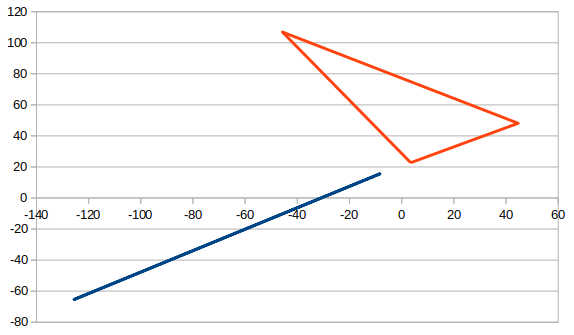
\includegraphics[width=10cm]{./degeneratedFrame.png}\\
\end{figure}
\end{center}

This case can be detected and avoided prior to the intersection test by checking the determinant of the frame: degenerated frames have a null determinant. In the example above the determinant of the first frame is equal to -0.001667.

\subsubsection{2D static}

\begin{scriptsize}
\begin{ttfamily}
\lstinputlisting[breaklines]{../Results/validation2D.txt}
\end{ttfamily}
\end{scriptsize}

\subsubsection{2D dynamic}

\begin{scriptsize}
\begin{ttfamily}
\lstinputlisting[breaklines]{../Results/validation2DTime.txt}
\end{ttfamily}
\end{scriptsize}

\subsubsection{3D static}

\begin{scriptsize}
\begin{ttfamily}
\lstinputlisting[breaklines]{../Results/validation3D.txt}
\end{ttfamily}
\end{scriptsize}

\subsubsection{3D dynamic}

\begin{scriptsize}
\begin{ttfamily}
\lstinputlisting[breaklines]{../Results/validation3DTime.txt}
\end{ttfamily}
\end{scriptsize}

\section{Qualification against SAT}

In this section I introduce the code I've used to qualify the algorithm and its implementation. The qualification consists of running the FMB algorithm on randomly generated pairs of Frame, and check its execution time against the one of running the SAT algorithm on the same pair of Frames.\\

\subsection{Code}

\subsubsection{2D static}

\begin{scriptsize}
\begin{ttfamily}
\lstinputlisting[breaklines,firstline=19]{../2D/qualification.c}
\end{ttfamily}
\end{scriptsize}

\subsubsection{3D static}

\begin{scriptsize}
\begin{ttfamily}
\lstinputlisting[breaklines,firstline=19]{../3D/qualification.c}
\end{ttfamily}
\end{scriptsize}

\subsubsection{2D dynamic}

\begin{scriptsize}
\begin{ttfamily}
\lstinputlisting[breaklines,firstline=19]{../2DTime/qualification.c}
\end{ttfamily}
\end{scriptsize}

\subsubsection{3D dynamic}

\begin{scriptsize}
\begin{ttfamily}
\lstinputlisting[breaklines,firstline=19]{../3DTime/qualification.c}
\end{ttfamily}
\end{scriptsize}

\subsection{Results}

In this subsection I give the results of the qualification for each case. These results are commented in the next section.\\

\clearpage
\subsubsection{2D static}

\begin{turn}{-90}
%\begin{adjustwidth}{-3cm}{-3.5cm}
\vbox{
\begin{tiny}
\begin{ttfamily}
\csvautotabular{../Results/qualification2D.txt}\\
\csvautotabular{../Results/qualification2DCC.txt}\\
\csvautotabular{../Results/qualification2DCT.txt}\\
\csvautotabular{../Results/qualification2DTC.txt}\\
\csvautotabular{../Results/qualification2DTT.txt}\\
\end{ttfamily}
\end{scriptsize}
}
%\end{adjustwidth}
\end{turn}

\begin{center}
\begin{figure}[H]
\centering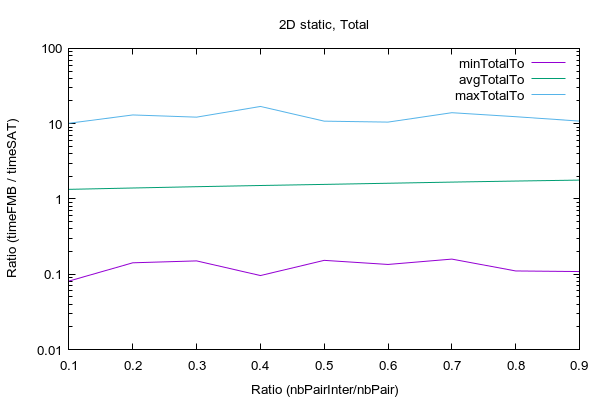
\includegraphics[width=12cm]{../Results/qualification2D.png}\\
\end{figure}
\end{center}

\begin{center}
\begin{figure}[H]
\centering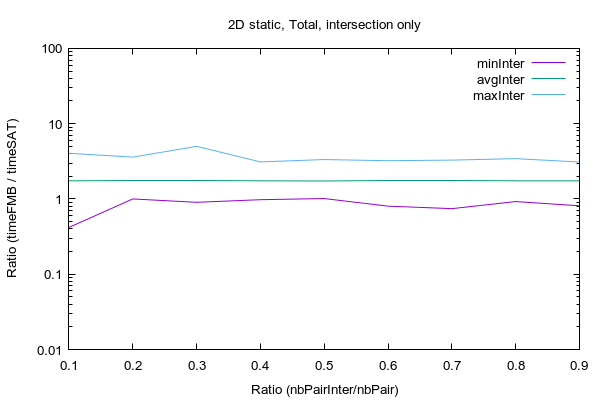
\includegraphics[width=12cm]{../Results/qualification2Dinter.png}\\
\centering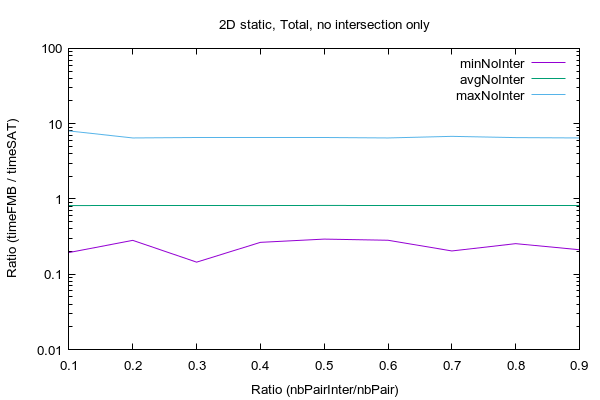
\includegraphics[width=12cm]{../Results/qualification2Dnointer.png}\\
\end{figure}
\end{center}
\begin{center}
\begin{figure}[H]
\centering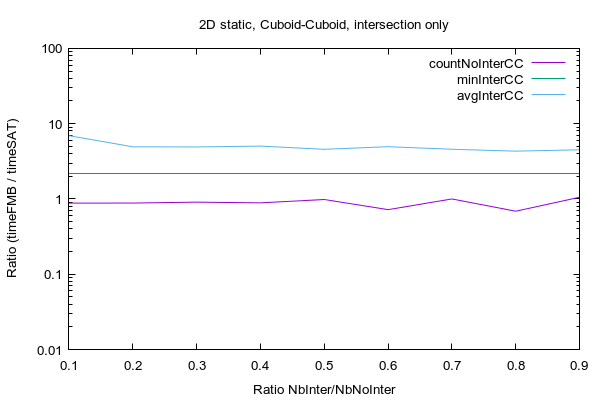
\includegraphics[width=7cm]{../Results/qualification2DCCinter.png}
\centering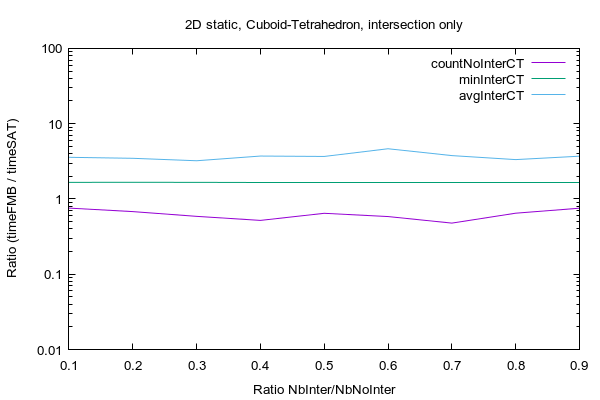
\includegraphics[width=7cm]{../Results/qualification2DCTinter.png}
\centering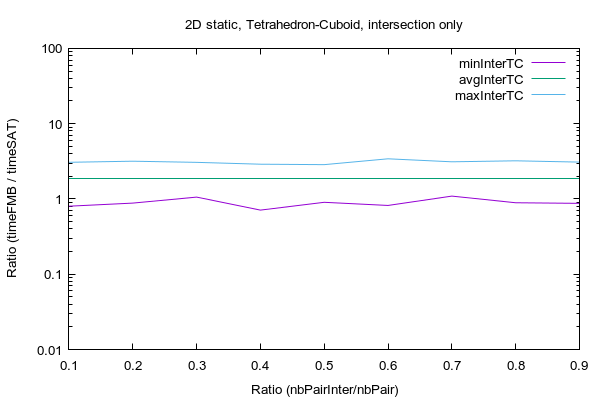
\includegraphics[width=7cm]{../Results/qualification2DTCinter.png}
\centering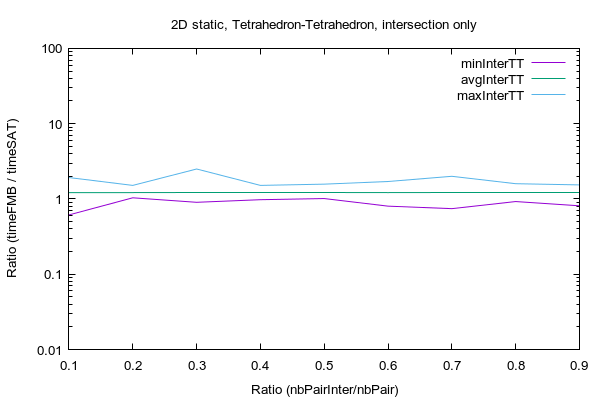
\includegraphics[width=7cm]{../Results/qualification2DTTinter.png}
\end{figure}
\end{center}
\begin{center}
\begin{figure}[H]
\centering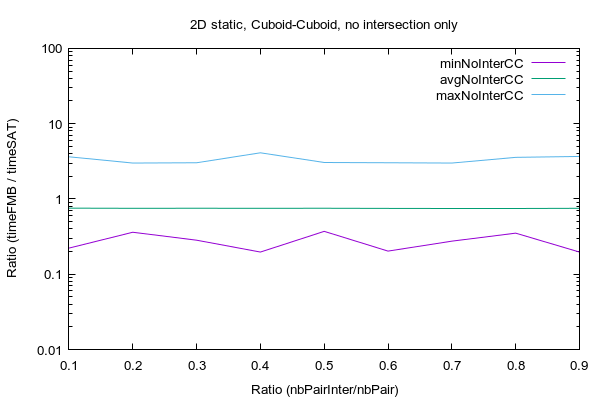
\includegraphics[width=7cm]{../Results/qualification2DCCnointer.png}
\centering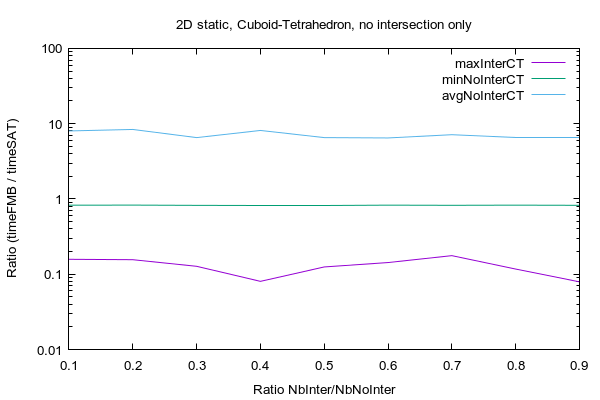
\includegraphics[width=7cm]{../Results/qualification2DCTnointer.png}
\centering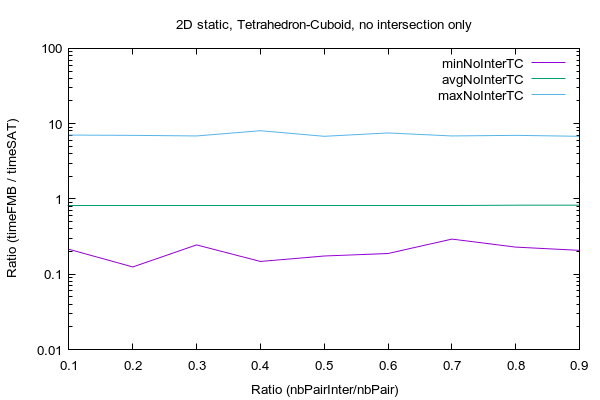
\includegraphics[width=7cm]{../Results/qualification2DTCnointer.png}
\centering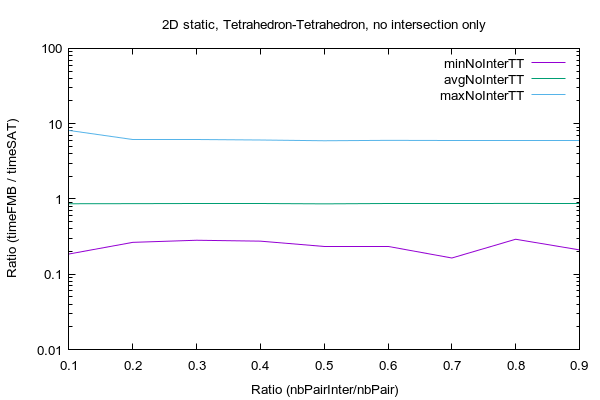
\includegraphics[width=7cm]{../Results/qualification2DTTnointer.png}
\end{figure}
\end{center}

\subsubsection{2D static (near case only)}

\begin{turn}{-90}
%\begin{adjustwidth}{-3cm}{-3.5cm}
\vbox{
\begin{tiny}
\begin{ttfamily}
\csvautotabular{../Results/qualification2Dnearcaseonly.txt}\\
\csvautotabular{../Results/qualification2DCCnearcaseonly.txt}\\
\csvautotabular{../Results/qualification2DCTnearcaseonly.txt}\\
\csvautotabular{../Results/qualification2DTCnearcaseonly.txt}\\
\csvautotabular{../Results/qualification2DTTnearcaseonly.txt}\\
\end{ttfamily}
\end{scriptsize}
}
%\end{adjustwidth}
\end{turn}

\begin{center}
\begin{figure}[H]
\centering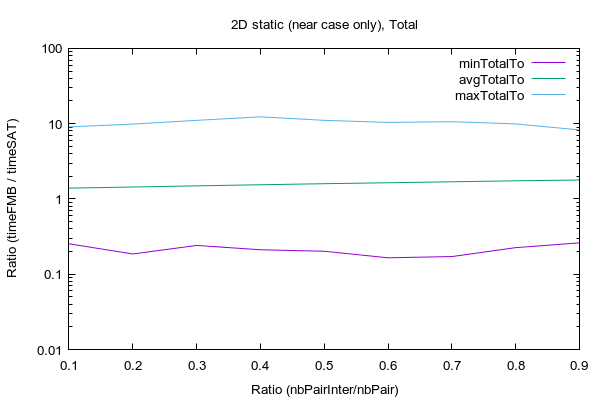
\includegraphics[width=12cm]{../Results/qualification2DNearCaseOnly.png}\\
\end{figure}
\end{center}

\begin{center}
\begin{figure}[H]
\centering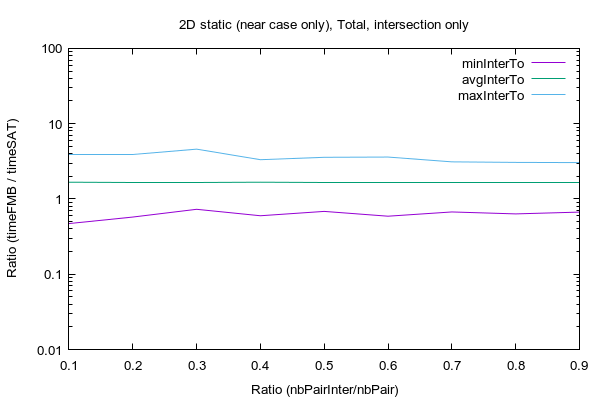
\includegraphics[width=12cm]{../Results/qualification2DinterNearCaseOnly.png}\\
\centering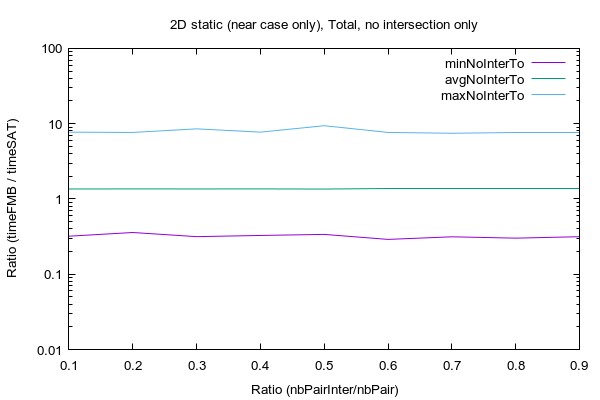
\includegraphics[width=12cm]{../Results/qualification2DnointerNearCaseOnly.png}\\
\end{figure}
\end{center}
\begin{center}
\begin{figure}[H]
\centering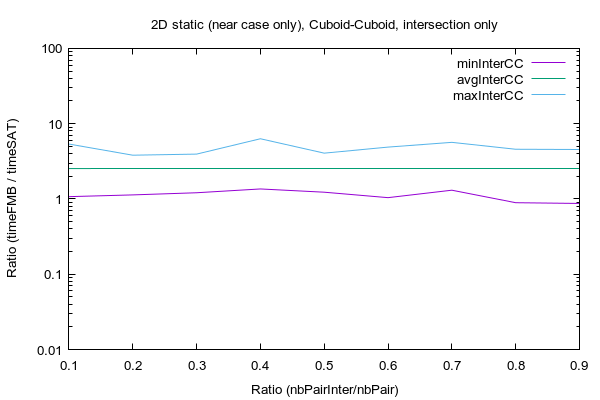
\includegraphics[width=7cm]{../Results/qualification2DCCinterNearCaseOnly.png}
\centering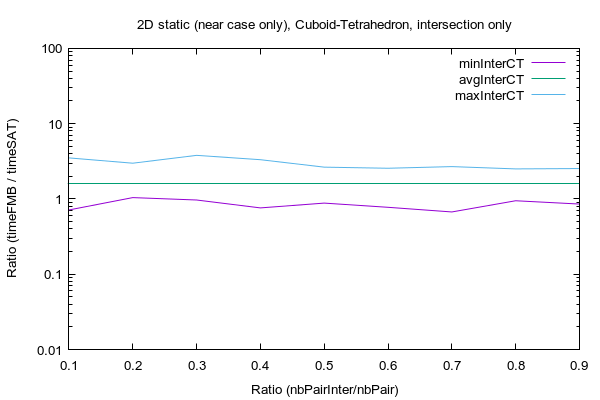
\includegraphics[width=7cm]{../Results/qualification2DCTinterNearCaseOnly.png}
\centering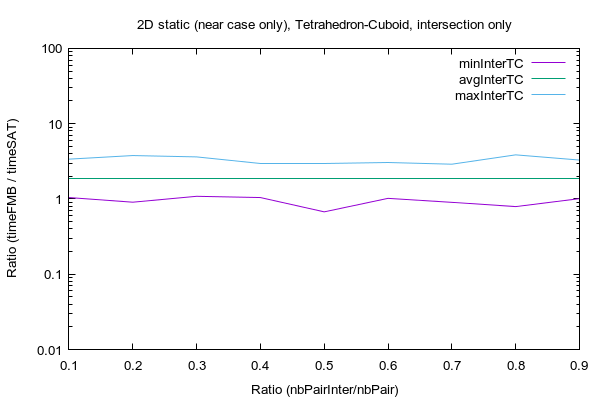
\includegraphics[width=7cm]{../Results/qualification2DTCinterNearCaseOnly.png}
\centering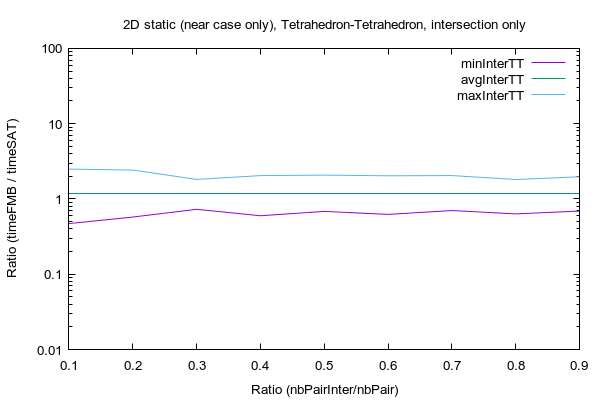
\includegraphics[width=7cm]{../Results/qualification2DTTinterNearCaseOnly.png}
\end{figure}
\end{center}
\begin{center}
\begin{figure}[H]
\centering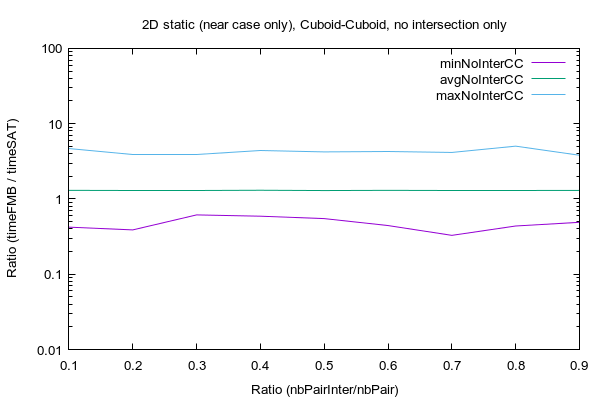
\includegraphics[width=7cm]{../Results/qualification2DCCnointerNearCaseOnly.png}
\centering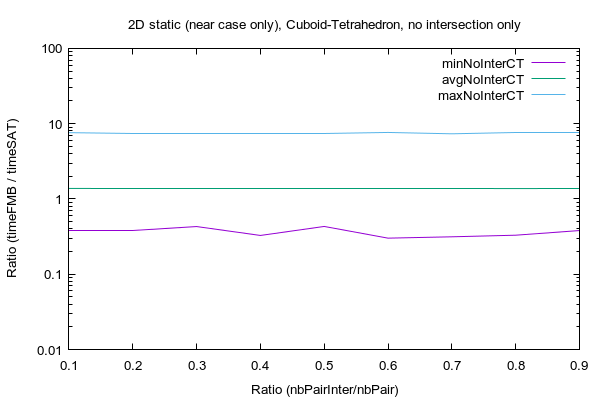
\includegraphics[width=7cm]{../Results/qualification2DCTnointerNearCaseOnly.png}
\centering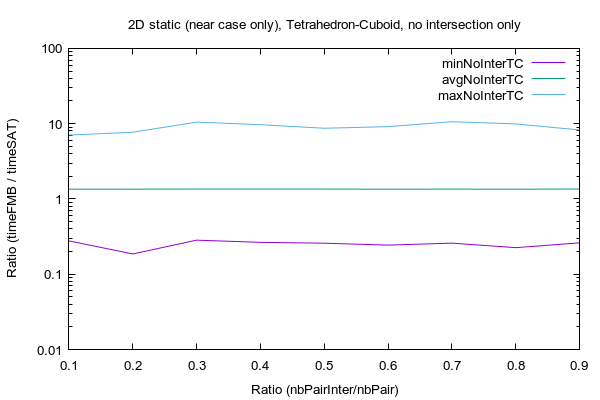
\includegraphics[width=7cm]{../Results/qualification2DTCnointerNearCaseOnly.png}
\centering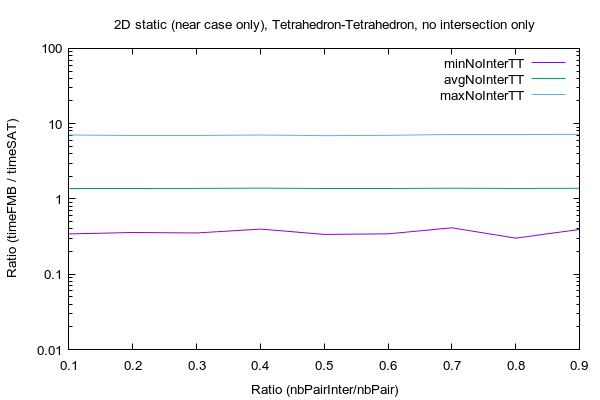
\includegraphics[width=7cm]{../Results/qualification2DTTnointerNearCaseOnly.png}
\end{figure}
\end{center}

\subsubsection{3D static}

\begin{turn}{-90}
%\begin{adjustwidth}{-3cm}{-3.5cm}
\vbox{
\begin{tiny}
\begin{ttfamily}
\csvautotabular{../Results/qualification3D.txt}\\
\csvautotabular{../Results/qualification3DCC.txt}\\
\csvautotabular{../Results/qualification3DCT.txt}\\
\csvautotabular{../Results/qualification3DTC.txt}\\
\csvautotabular{../Results/qualification3DTT.txt}\\
\end{ttfamily}
\end{scriptsize}
}
%\end{adjustwidth}
\end{turn}

\begin{center}
\begin{figure}[H]
\centering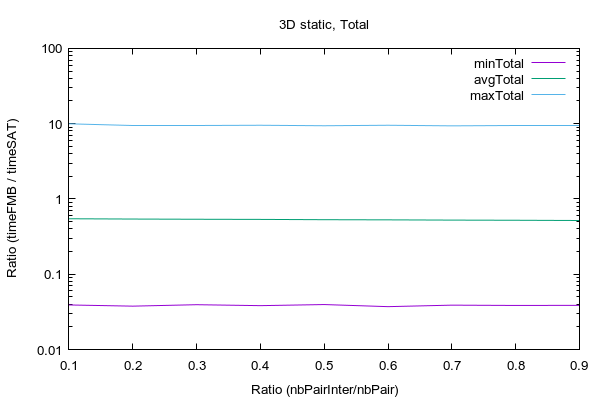
\includegraphics[width=12cm]{../Results/qualification3D.png}\\
\end{figure}
\end{center}

\begin{center}
\begin{figure}[H]
\centering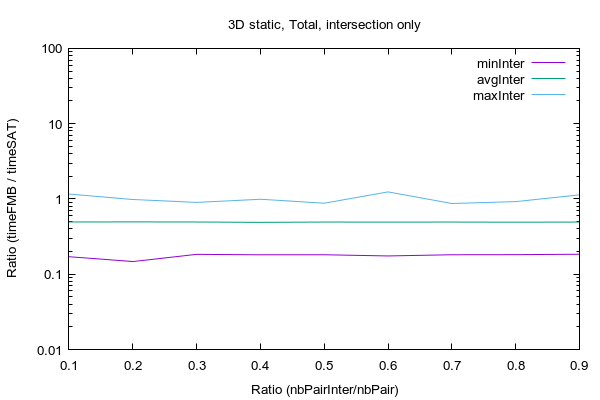
\includegraphics[width=12cm]{../Results/qualification3Dinter.png}\\
\centering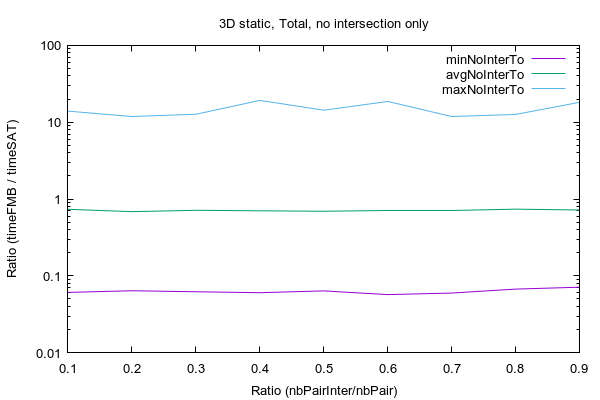
\includegraphics[width=12cm]{../Results/qualification3Dnointer.png}\\
\end{figure}
\end{center}
\begin{center}
\begin{figure}[H]
\centering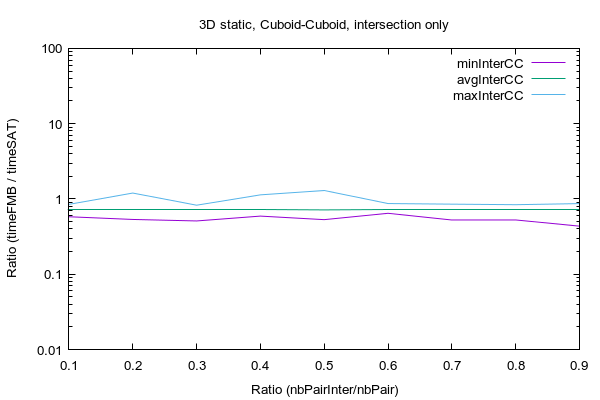
\includegraphics[width=7cm]{../Results/qualification3DCCinter.png}
\centering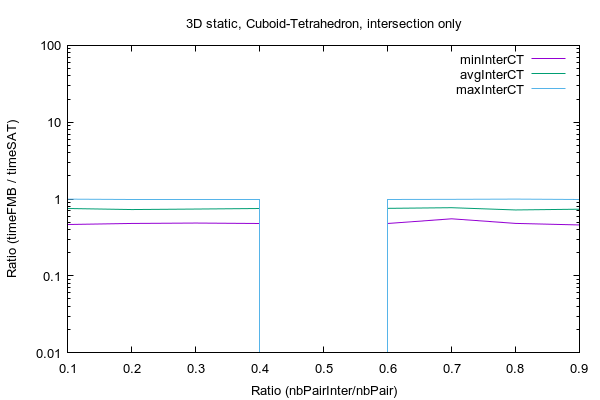
\includegraphics[width=7cm]{../Results/qualification3DCTinter.png}
\centering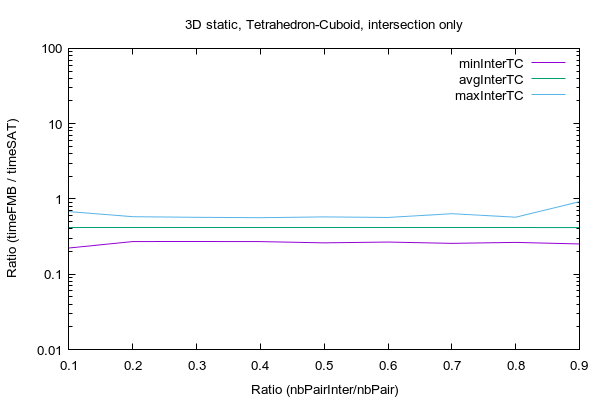
\includegraphics[width=7cm]{../Results/qualification3DTCinter.png}
\centering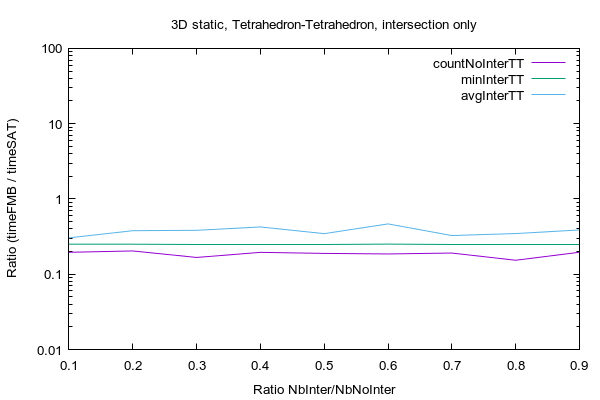
\includegraphics[width=7cm]{../Results/qualification3DTTinter.png}
\end{figure}
\end{center}
\begin{center}
\begin{figure}[H]
\centering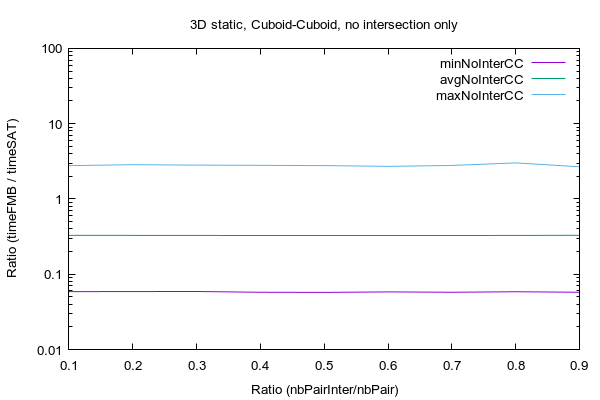
\includegraphics[width=7cm]{../Results/qualification3DCCnointer.png}
\centering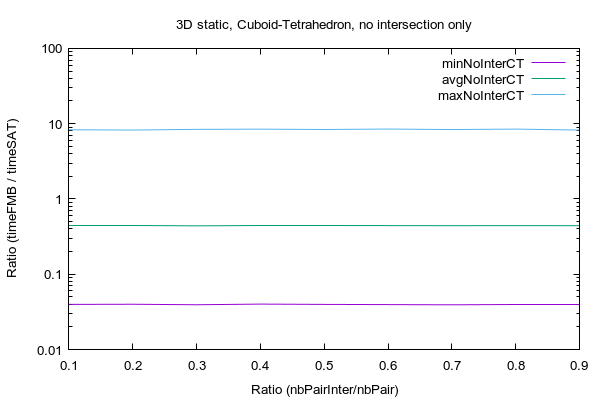
\includegraphics[width=7cm]{../Results/qualification3DCTnointer.png}
\centering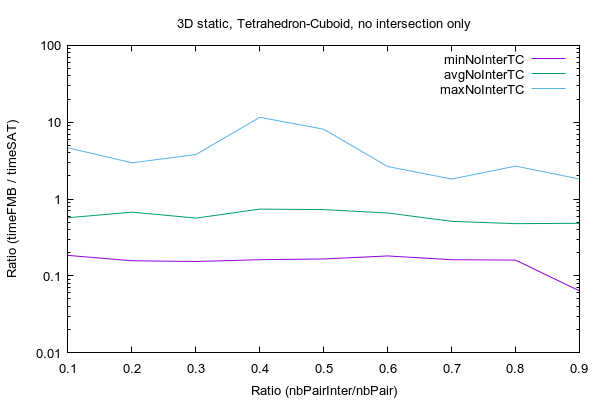
\includegraphics[width=7cm]{../Results/qualification3DTCnointer.png}
\centering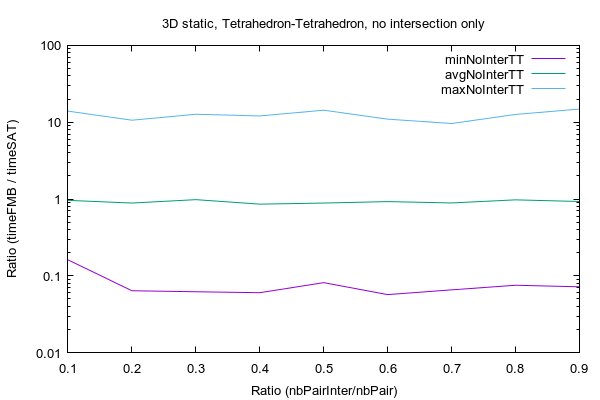
\includegraphics[width=7cm]{../Results/qualification3DTTnointer.png}
\end{figure}
\end{center}

\subsubsection{3D static (near case only)}

\begin{turn}{-90}
%\begin{adjustwidth}{-3cm}{-3.5cm}
\vbox{
\begin{tiny}
\begin{ttfamily}
\csvautotabular{../Results/qualification3Dnearcaseonly.txt}\\
\csvautotabular{../Results/qualification3DCCnearcaseonly.txt}\\
\csvautotabular{../Results/qualification3DCTnearcaseonly.txt}\\
\csvautotabular{../Results/qualification3DTCnearcaseonly.txt}\\
\csvautotabular{../Results/qualification3DTTnearcaseonly.txt}\\
\end{ttfamily}
\end{scriptsize}
}
%\end{adjustwidth}
\end{turn}

\begin{center}
\begin{figure}[H]
\centering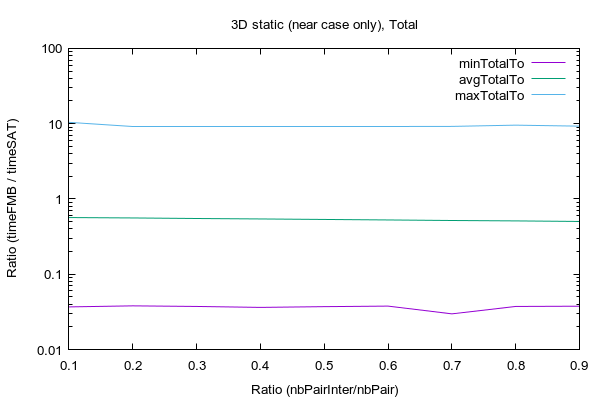
\includegraphics[width=12cm]{../Results/qualification3DNearCaseOnly.png}\\
\end{figure}
\end{center}

\begin{center}
\begin{figure}[H]
\centering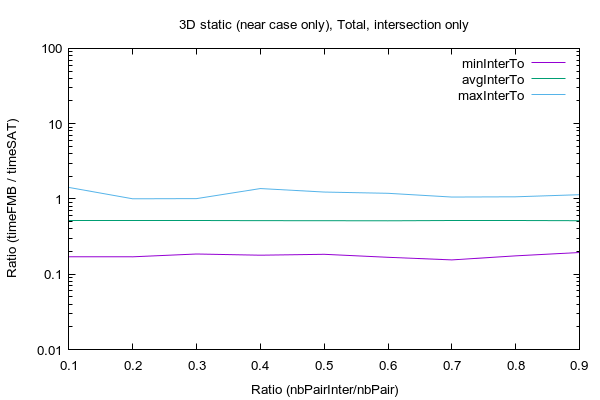
\includegraphics[width=12cm]{../Results/qualification3DinterNearCaseOnly.png}\\
\centering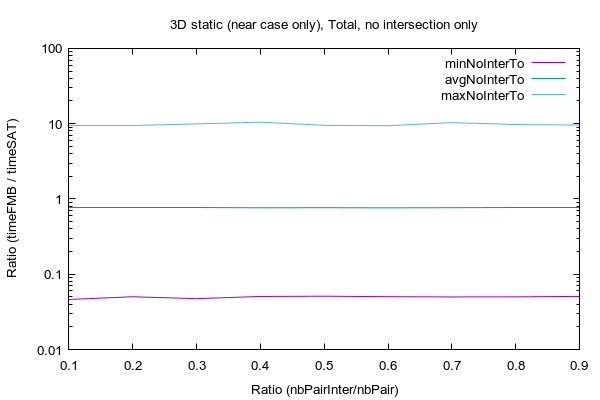
\includegraphics[width=12cm]{../Results/qualification3DnointerNearCaseOnly.png}\\
\end{figure}
\end{center}
\begin{center}
\begin{figure}[H]
\centering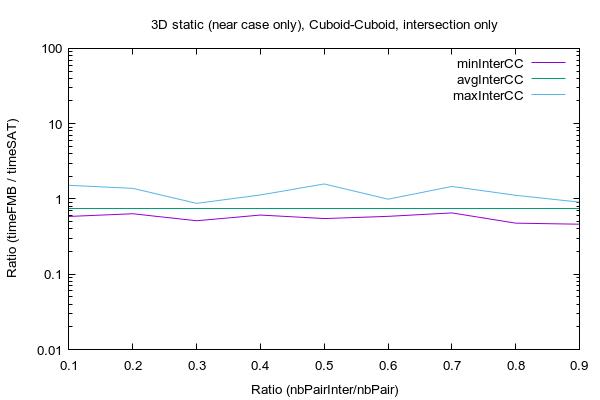
\includegraphics[width=7cm]{../Results/qualification3DCCinterNearCaseOnly.png}
\centering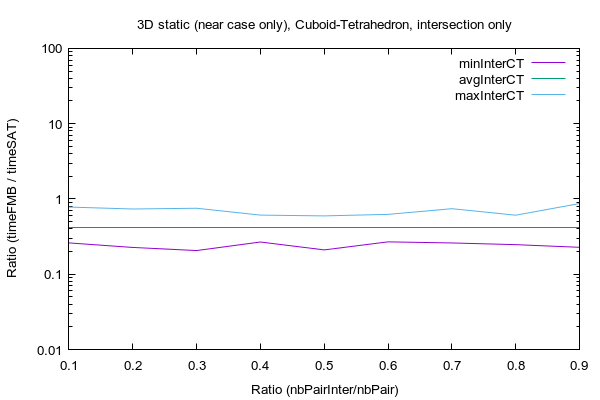
\includegraphics[width=7cm]{../Results/qualification3DCTinterNearCaseOnly.png}
\centering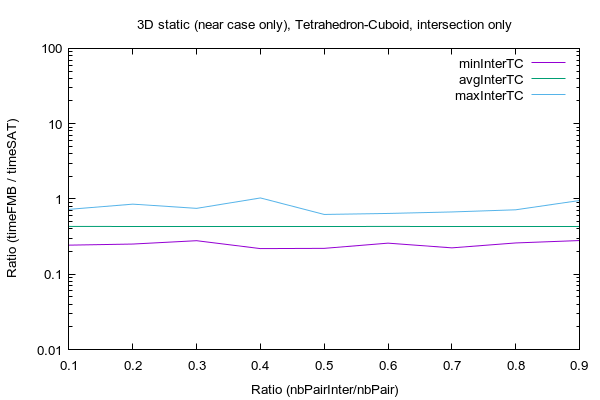
\includegraphics[width=7cm]{../Results/qualification3DTCinterNearCaseOnly.png}
\centering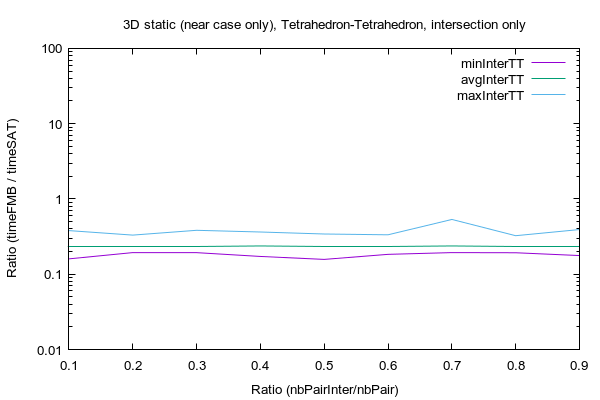
\includegraphics[width=7cm]{../Results/qualification3DTTinterNearCaseOnly.png}
\end{figure}
\end{center}
\begin{center}
\begin{figure}[H]
\centering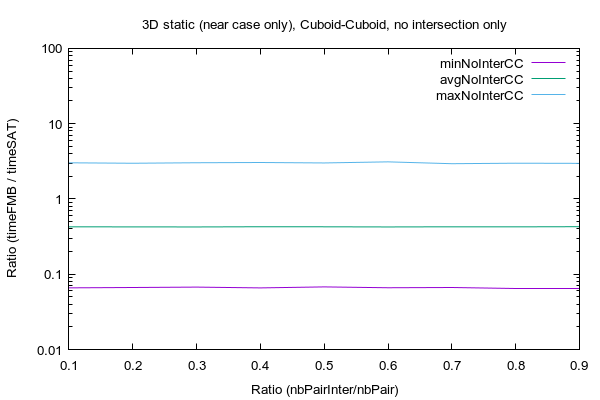
\includegraphics[width=7cm]{../Results/qualification3DCCnointerNearCaseOnly.png}
\centering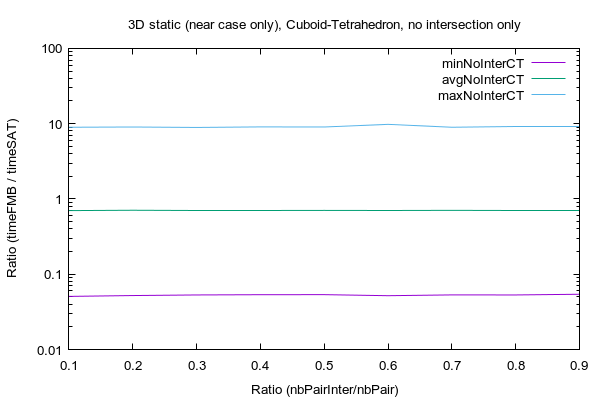
\includegraphics[width=7cm]{../Results/qualification3DCTnointerNearCaseOnly.png}
\centering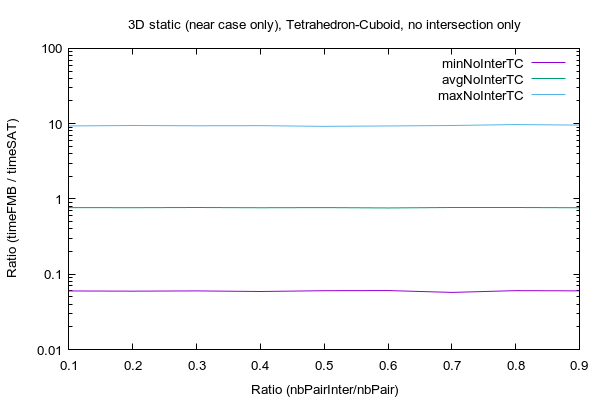
\includegraphics[width=7cm]{../Results/qualification3DTCnointerNearCaseOnly.png}
\centering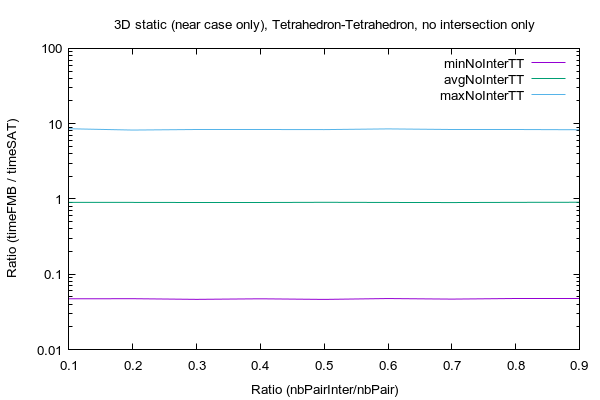
\includegraphics[width=7cm]{../Results/qualification3DTTnointerNearCaseOnly.png}
\end{figure}
\end{center}

\subsubsection{2D dynamic}

\begin{turn}{-90}
%\begin{adjustwidth}{-3cm}{-3.5cm}
\vbox{
\begin{tiny}
\begin{ttfamily}
\csvautotabular{../Results/qualification2DTime.txt}\\
\csvautotabular{../Results/qualification2DTimeCC.txt}\\
\csvautotabular{../Results/qualification2DTimeCT.txt}\\
\csvautotabular{../Results/qualification2DTimeTC.txt}\\
\csvautotabular{../Results/qualification2DTimeTT.txt}\\
\end{ttfamily}
\end{scriptsize}
}
%\end{adjustwidth}
\end{turn}

\begin{center}
\begin{figure}[H]
\centering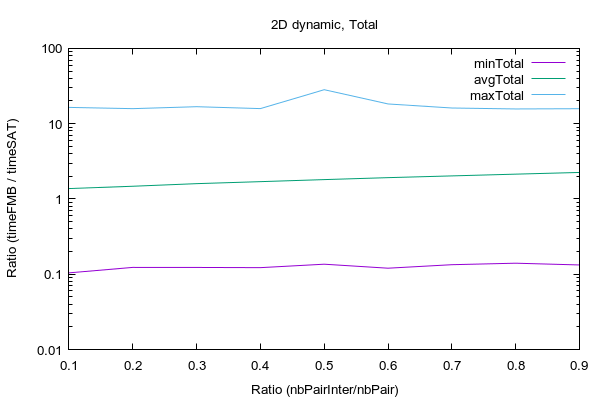
\includegraphics[width=12cm]{../Results/qualification2DTime.png}\\
\end{figure}
\end{center}

\begin{center}
\begin{figure}[H]
\centering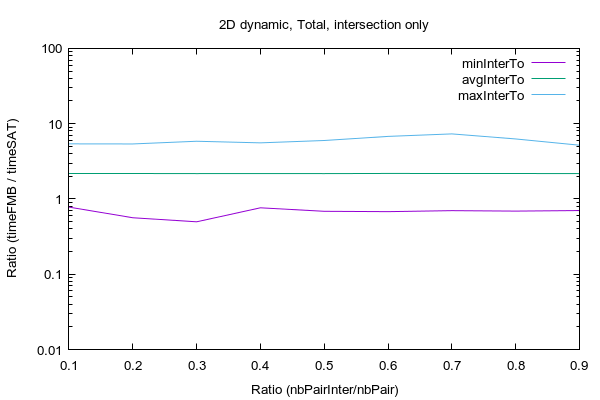
\includegraphics[width=12cm]{../Results/qualification2DTimeinter.png}\\
\centering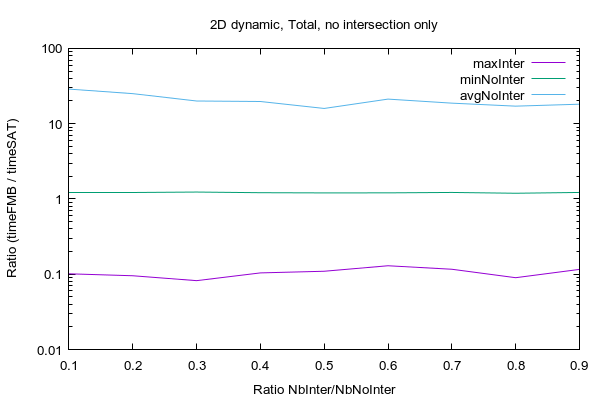
\includegraphics[width=12cm]{../Results/qualification2DTimenointer.png}\\
\end{figure}
\end{center}
\begin{center}
\begin{figure}[H]
\centering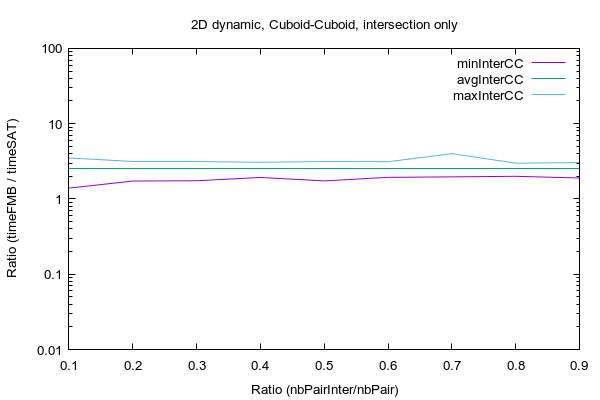
\includegraphics[width=7cm]{../Results/qualification2DTimeCCinter.png}
\centering\includegraphics[width=7cm]{../Results/qualification2DTimeCTinter.png}
\centering\includegraphics[width=7cm]{../Results/qualification2DTimeTCinter.png}
\centering\includegraphics[width=7cm]{../Results/qualification2DTimeTTinter.png}
\end{figure}
\end{center}
\begin{center}
\begin{figure}[H]
\centering\includegraphics[width=7cm]{../Results/qualification2DTimeCCnointer.png}
\centering\includegraphics[width=7cm]{../Results/qualification2DTimeCTnointer.png}
\centering\includegraphics[width=7cm]{../Results/qualification2DTimeTCnointer.png}
\centering\includegraphics[width=7cm]{../Results/qualification2DTimeTTnointer.png}
\end{figure}
\end{center}

\subsubsection{3D dynamic}

\begin{turn}{-90}
%\begin{adjustwidth}{-3cm}{-3.5cm}
\vbox{
\begin{tiny}
\begin{ttfamily}
\csvautotabular{../Results/qualification3DTime.txt}\\
\csvautotabular{../Results/qualification3DTimeCC.txt}\\
\csvautotabular{../Results/qualification3DTimeCT.txt}\\
\csvautotabular{../Results/qualification3DTimeTC.txt}\\
\csvautotabular{../Results/qualification3DTimeTT.txt}\\
\end{ttfamily}
\end{scriptsize}
}
%\end{adjustwidth}
\end{turn}

\begin{center}
\begin{figure}[H]
\centering\includegraphics[width=12cm]{../Results/qualification3DTime.png}\\
\end{figure}
\end{center}

\begin{center}
\begin{figure}[H]
\centering\includegraphics[width=12cm]{../Results/qualification3DTimeinter.png}\\
\centering\includegraphics[width=12cm]{../Results/qualification3DTimenointer.png}\\
\end{figure}
\end{center}
\begin{center}
\begin{figure}[H]
\centering\includegraphics[width=7cm]{../Results/qualification3DTimeCCinter.png}
\centering\includegraphics[width=7cm]{../Results/qualification3DTimeCTinter.png}
\centering\includegraphics[width=7cm]{../Results/qualification3DTimeTCinter.png}
\centering\includegraphics[width=7cm]{../Results/qualification3DTimeTTinter.png}
\end{figure}
\end{center}
\begin{center}
\begin{figure}[H]
\centering\includegraphics[width=7cm]{../Results/qualification3DTimeCCnointer.png}
\centering\includegraphics[width=7cm]{../Results/qualification3DTimeCTnointer.png}
\centering\includegraphics[width=7cm]{../Results/qualification3DTimeTCnointer.png}
\centering\includegraphics[width=7cm]{../Results/qualification3DTimeTTnointer.png}
\end{figure}
\end{center}

\section{Comments about the qualification results}

For the 2D static case:\\

\begin{itemize}
\item FMB is in average 1.3 times slower than SAT to detect intersection and non intersection between Tetrahedrons.\\
\item FMB is in average 1.9 times slower than SAT to detect intersection between a Tetrahedron and a Cuboid, and 1.3 times slower to detect non intersection.\\
\item FMB is in average 2.5 times slower than SAT to detect intersection between Cuboids, and 1.2 times slower to detect non intersection.\\
\end{itemize}

FMB is then in average always slower (from 2.5 times to 1.2 times) than SAT whatever the combinaison of Tetrahedron and Cuboid and the percentage of intersection.\\ 

For the 3D static case:\\

\begin{itemize}
\item FMB is in average 4.2 times faster than SAT to detect intersection between Tetrahedrons, and 1.1 times faster to detect non intersection.\\
\item FMB is in average 2.4 times faster than SAT to detect intersection between a Tetrahedron and a Cuboid, and 1.5 times faster to detect non intersection.\\
\item FMB is in average 1.4 times faster than SAT to detect intersection between Cuboids, and 2.0 times faster to detect non intersection.\\
\end{itemize}

FMB is then in average always faster (from 4.2 times to 1.1 times) than SAT whatever the combinaison of Tetrahedron and Cuboid and the percentage of intersection.\\ 

For the 2D dynamic case:\\

\begin{itemize}
\item FMB is in average 1.7 times slower than SAT to detect intersection between Tetrahedrons, and 1.5 times slower to detect non intersection.\\
\item FMB is in average 2.2 times slower than SAT to detect intersection between a Tetrahedron and a Cuboid, and 1.5 times slower to detect non intersection.\\
\item FMB is in average 3.1 times slower than SAT to detect intersection between Cuboids, and 1.5 times slower to detect non intersection.\\
\end{itemize}

FMB is then in average always slower (from 3.1 times to 1.5 times) than SAT whatever the combinaison of Tetrahedron and Cuboid and the percentage of intersection.\\ 

For the 3D dynamic case:\\

\begin{itemize}
\item FMB is in average 1.8 times faster than SAT to detect intersection between Tetrahedrons, and 1.05 times faster to detect non intersection.\\
\item FMB is in average 1.4 times slower than SAT to detect intersection between a Tetrahedron and a Cuboid, and 1.2 times faster to detect non intersection.\\
\item FMB is in average 2.6 times slower than SAT to detect intersection between Cuboids, and 1.4 times faster to detect non intersection.\\
\end{itemize}

FMB is then in average always faster (from 1.8 times to 1.05 times) than SAT for a set of Tetrahedron, and faster than SAT for a combinaison of Tetrahedrons and Cuboids containining less than around 35\% of intersection, or a combinaison of Cuboids containining less than around 15\% of intersection.\\ 

Overall, FMB is faster than SAT, at least if the percentage of intersecting Frames is low, for the 3D cases. But it is always slower for the 2D dynamic cases. In practice, for example in applications where the Frames represents real world objects supposedly normally not in intersection, FMB would be a better choice than SAT for 3D applications.\\

In a real world collision detection system the pair of Frames would be pruned by first applying a rough but fast detection algorithm. The slower but accurate SAT and FMB algorithms would be then only applied to pairs of Frames closed together. To ensure the results stay valid on this subset of possible cases, I've also run the qualification for 2D and 3D static cases in 'near case only' mode. In this mode, only pairs of Frames whose AABBs are intersecting are used. The results are as follow.\\

For the 2D static near only case:\\

\begin{itemize}
\item FMB is in average 1.3 times slower than SAT to detect intersection between Tetrahedrons, and 1.4 times slower to detect non intersection.\\
\item FMB is in average 1.9 times slower than SAT to detect intersection between a Tetrahedron and a Cuboid, and 1.4 times slower to detect non intersection.\\
\item FMB is in average 2.5 times slower than SAT to detect intersection between Cuboids, and 1.3 times slower to detect non intersection.\\
\end{itemize}

There is no significant difference with the general cases.\\ 

For the 3D static near only case:\\

\begin{itemize}
\item FMB is in average 4.3 times faster than SAT to detect intersection between Tetrahedrons, and 1.1 times faster to detect non intersection.\\
\item FMB is in average 2.4 times faster than SAT to detect intersection between a Tetrahedron and a Cuboid, and 1.5 times faster to detect non intersection.\\
\item FMB is in average 1.4 times faster than SAT to detect intersection between Cuboids, and 2.0 times faster to detect non intersection.\\
\end{itemize}

There is no significant difference with the general cases.\\ 

SAT and FMB follows the same strategy: assume that the pair of Frames is in intersection and try to prove it is false by checking a list of conditions. These conditions are the difference between the two algorithms. The results of the qualification show that in average the conditions used by FMB allows to detect a non intersection faster than those of SAT.\\

For one given pair in intersection, all the conditions must be checked before the algorithms give their answer. The algorithm with the smallest execution time of all these conditions is then the fastest, and the results shows that this is in general SAT (the exceptions are the 3D static case and 3D dynamic case for Tetrahedrons pairs). This is shown in the results by the low variability of the ratio timeFMB/timeSAT for intersecting pairs.\\

For one given pair not in intersection, the algorithms reply as soon as one condition is verified. This may be the first one, as it may be the last one depending on the geometry of the pair of Frames. Then, the variability of the ratio timeFMB/timeSAT varies widely as shown in the results, from 50 times faster to 29 times slower, but the resuts shows that in general the advantage goes to the FMB algorithm (the exception is the 2D dynamic case).\\

In the SAT algorithm, one must perform the projection of all vertices on one axis and then check the result which is the intersection condition. Every axis comes from the geometry of the Frames and one cannot preview which one will be lead to the checked condition for a non intersecting pair. In the FMB algorithm, the conditions depends on the way the system of linear inequation is built. Then, for best performances, it must be done in such a way that inequality (\ref{cond_non_intersec}) is encountered as soon as possible. With the FMB representation, contrary to the SAT one, it is possible to do so independantly of the geometry of the pair of Frames by reordering the inequalities of the system. For example, the $X_i\le1.0$ inequalities must be moved down to the end of the system of the linear inequalities for better performance, as they will never lead to '(\ref{cond_non_intersec}) is true' at the first step of the Fourier-Motzkin algorithm.\\

Looking for other rearrangement of the inequations, I've come to the conclusion that the best possible case (in term of speed) is, when checking Frame A against Frame B, to have:\\
\begin{itemize}
\item B's origin is the nearest vertex of B relative to A's origin
\item the projection of B's origin in A's coordinate system is such as components of $\overrightarrow{AB_A}$ are all positive
\end{itemize}
This the best possible case because it minimised the $a_i$ in (\ref{cond_non_intersec}) in the initial system or during Fourier-Motzkin algorithm, which leads quickly to '(\ref{cond_non_intersec}) is true' if the Frames are not in intersection. The Frame representation is invariant of the vertex choosen as origin, so it's possible to rearrange them to try to fit the conditions above (however it's not always possible to fit both). I've checked that it effectively leads to slightly better performances by first modifying the qualification program to generate only these cases, and then by adding a rearrangement of the origins at the beginning of the FMB algorithm. Unfortunately, the cost of the origin rearrangement is heavier than its benefit. Still, I believe one may find some clever rearrangement which would lead to even better performance for the FMB algorithm.\\

\section{Conclusion}

In this paper I've introduced the FMB algorithm which solve efficiently the intersection detection problem of 2D/3D static/dynamic cuboid/tetrahedron by using the Fourier-Motzkin elimination method. All information necessary to implement and use the FMB algorithm, or reproduce the results introduced in this paper are included in this paper, and available on the GitHub repository https://github.com/BayashiPascal/FMB/ .\\

Validation and qualification against the SAT algorithm prove the correctness of the results from the FMB algorithm and prove it's a valid alternative in term of performance to the SAT algorithm, especially when applied to tetrahedrons and/or in the 3D static case. It is also important to note its simplicity to implement, and the fact that the FMB algorithm returns a bounding box of the intersection, if any, while the SAT algorithm only returns a boolean answer.\\

Idea on direction to explore with the view to improve the FMB algorithm is given. Steps of the Fourier-Motzkin could also be easily parallelized on an appropriate architecture to improve performance. Tests of implementation with others programming languages, or on other runtime environments, or against other algorithms (such as CJK) would also be interesting to perform. Finally, while the algorithm is introduced here in 2D and 3D, its extension to upper dimensions is straightforward.\\

\section{Annex}

\subsection{Runtime environment}
\label{runtime_environment}

Results introduce in this paper have been produced by compiling and running the corresponding algorithms in the following environment:\\

\begin{scriptsize}
\begin{ttfamily}
\lstinputlisting[breaklines]{../runtimeEnv.txt}
\end{ttfamily}
\end{scriptsize}


\subsection{SAT implementation}
\label{sat_implementation}

In this section I introduce the code of the implementation of the SAT algorithm, used to validate and qualify the FMB algorithm.\\

\subsubsection{Header}

\begin{scriptsize}
\begin{ttfamily}
\lstinputlisting[breaklines,firstline=19]{../SAT/sat.h}
\end{ttfamily}
\end{scriptsize}

\subsubsection{Body}

\begin{scriptsize}
\begin{ttfamily}
\lstinputlisting[breaklines,firstline=19]{../SAT/sat.c}
\end{ttfamily}
\end{scriptsize}

\subsection{Makefile}

In this section I introduce the Makefile used to compile the code given in the previous sections. It also includes command used to run the unit tests, validation and qualification, and to generate the documentation.\\

\begin{scriptsize}
\begin{ttfamily}
\lstinputlisting[breaklines]{../Makefile}
\end{ttfamily}
\end{scriptsize}

\subsubsection{2D static}

\begin{scriptsize}
\begin{ttfamily}
\lstinputlisting[breaklines]{../2D/Makefile}
\end{ttfamily}
\end{scriptsize}

\subsubsection{3D static}

\begin{scriptsize}
\begin{ttfamily}
\lstinputlisting[breaklines]{../3D/Makefile}
\end{ttfamily}
\end{scriptsize}

\subsubsection{2D dynamic}

\begin{scriptsize}
\begin{ttfamily}
\lstinputlisting[breaklines]{../2DTime/Makefile}
\end{ttfamily}
\end{scriptsize}

\subsubsection{3D dynamic}

\begin{scriptsize}
\begin{ttfamily}
\lstinputlisting[breaklines]{../3DTime/Makefile}
\end{ttfamily}
\end{scriptsize}

\subsubsection{Doc}

\begin{scriptsize}
\begin{ttfamily}
\lstinputlisting[breaklines]{../Doc/Makefile}
\end{ttfamily}
\end{scriptsize}

\subsection{Dynamic analysis}

\begin{scriptsize}
\begin{ttfamily}
\lstinputlisting[breaklines]{../dynamicAnalysis.txt}
\end{ttfamily}
\end{scriptsize}

\subsection{Static analysis}

\begin{scriptsize}
\begin{ttfamily}
\lstinputlisting[breaklines]{../staticAnalysis.txt}
\end{ttfamily}
\end{scriptsize}

\subsection{Versions of this paper}

This paper has been revised has follow:

\begin{itemize}
\item February 5th, 2020 : Original version
\item April 5th, 2020 : Addition of the 'near-case only' results in qualification.
\item April 25th, 2020 : Update of the qualification results after moving the computation of the inverse of components matrix from outside to inside the intersection detection test for a better comparison with SAT.
\item May 6th, 2020 : Add image on the first page. Correct erroneous indices notation in the formulation of the problem. Add generic algorithm.
\end{itemize}

\begin{thebibliography}{9}
\bibitem{fourier} J.J.-B. Fourier. Oeuvres II. Paris, 1890
\bibitem{motzkin} T.S. Motzkin. {\em Beitr\"{a}ge zur Theorie der linearen Ungleichungen}. Thesis, 1936. Reprinted in: {\em Theodore S. Motzkin: selected papers} (D.Cantor et al., eds,), Birkh\"{a}user, Boston, 1983.
\end{thebibliography}

\end{document}
